% !TEX encoding = windows-1250
\documentclass[12pt, oneside, a4paper]{mwbk}
\usepackage[cp1250]{inputenc}
\usepackage[polish]{babel}
\usepackage[OT4]{fontenc}

\usepackage{listings}
\lstset
{
	captionpos=b,
	basicstyle=\footnotesize\ttfamily,
	frame = single,
	tabsize = 3,
	breaklines = true
}
\renewcommand\lstlistlistingname{Spis listing�w}

\usepackage{graphicx}
\usepackage{verbatim}

\usepackage{enumitem}
\usepackage[noend]{algorithmic}
\usepackage[ruled]{algorithm}

\usepackage{color}
\usepackage[normalem]{ulem}

\usepackage{rotating}
\usepackage{float}
\usepackage{textpos}

\linespread{1,3}
\oddsidemargin = 10pt
\textwidth = 470pt

\hyphenpenalty=1000
\tolerance=500

\begin{document}
\author{Krzysztof Szczech}
\title{Tytu�}
\begin{titlepage}
\thispagestyle{empty}
\begin{textblock}{1}(-2.65,-1.65)

\includegraphics{figures/tytulowa_pusta_mgrinz.pdf}
\end{textblock}
\vspace{7.3cm}
\begin{center}
\fontfamily{ptm}
\selectfont
\Huge
Wybrane aspekty techniczne odwzorowania artystycznej wizji jako tr�jwymiarowego �rodowiska w grze komputerowej
\end{center}
\begin{center}
\fontfamily{ptm}
\selectfont
Praca dyplomowa in�ynierska
\end{center}
\vspace{5.6cm}
\begin{center}
\fontfamily{ptm}
\selectfont
\hspace{-1cm}
\begin{tabular}{l}
Wydzia� Fizyki Technicznej, Informatyki i Matematyki Stosowanej \\
Promotor: dr in�. Rafa� Szrajber \\
Dyplomant: Krzysztof Szczech \\
Nr albumu: 180707 \\
Kierunek: Informatyka \\
Specjalno��: Technologie gier i symulacji komputerowych
\end{tabular}
\end{center}
\vspace{-.5cm}
\begin{center}
\fontfamily{ptm}
\selectfont
\begin{textblock}{13}(0,0.2)
��d�, 2016
\end{textblock}
\end{center}
\end{titlepage}

\tableofcontents

% !TeX encoding = windows-1250

\chapter{Wst�p}
\label{t:introduction}
Bardzo szybki - trwaj�cy od kilku dziesi�cioleci - rozw�j komputer�w pozwoli� na przenoszenie coraz bardziej z�o�onych fragment�w otaczaj�cego nas �wiata na ekrany monitor�w. Jeste�my w stanie symulowa� skomplikowane zjawiska przyrody, co pozwala nam lepiej zrozumie� �wiat na kt�rym �yjemy, "budowa�"  wirtualne domy w kt�rych kiedy� b�dziemy chcieli zamieszka� w rzeczywisto�ci, czy te� tworzy� obrazy bez pomocy p��tna i p�dzla.\newline
W latach 90. XX wieku zacz�to tworzy� pierwsze gry komputerowe wykorzystuj�ce wielok�tow� grafik� tr�jwymiarow� \cite{MostInfluentialGames}. By� to pocz�tek nowej ery dla elektronicznej rozrywki. Pocz�tkowo liczba wielok�t�w by�a niska, a obraz by� renderowany w niewielkiej rozdzielczo�ci. Wraz z pojawianiem si� nowych akcelerator�w 3D liczby te zacz�y si� zwi�ksza�, co poprawia�o og�ln� jako�� grafiki. \newline 
Jednak po dzi� dzie� - mimo znacz�cego skoku technologicznego - pozosta� problem optymalnego tworzenia modeli i tekstur do gier w taki spos�b, aby komputer by� w stanie wytworzy� odpowiedni� liczb� klatek obrazu na sekund�. Przez lata rozwoju silnik�w graficznych  prze�cigano si� w pomys�ach na to, jak tworzy� assety (tr�jwymiarowe modele, tekstury, materia�y i animacje) aby wygl�da�y jak najatrakcyjniej dla gracza i jednocze�nie ich wykorzystywanie wymaga�o jak najmniejszej ilo�ci zasob�w komputera - w szczeg�lno�ci pami�ci RAM karty graficznej. Przy �le rozplanowanym procesie tw�rczym mo�e doj�� do sytuacji w kt�rej znacznie wyd�u�y si� czas oczekiwania na wczytanie z dysku twardego wszystkich wymaganych plik�w lub - w bardziej skrajnych przypadkach - karta graficzna komputera nie b�dzie nad��a�a z odpowiednio szybkim wytwarzaniem klatek animacji - co w znacznym stopniu zmniejszy komfort rozgrywki oraz poziom imersji gracza. Odpowiedni balans mi�dzy wspomnianymi aspektami jest jednym z najwi�kszych wyzwa� przed jakimi stawiani s� tw�rcy grafiki komputerowej wykorzystywanej w grach. \newpage
\section{Cel i za�o�enia pracy}
Celem pracy jest przedstawienie procesu tworzenia paczki modeli oraz tekstur na podstawie grafiki koncepcyjnej, kt�re jednocze�nie s� gotowe do wykorzystania w silniku gry komputerowej. Dodatkowo - szczeg�lny nacisk zosta� po�o�ony na techniczne aspekty tego procesu - w szczeg�lno�ci jak najlepsze wykorzystanie pami�ci operacyjnej komputera oraz odpowiednie zaplanowanie pracy w taki spos�b, aby mo�na by�a j� wykonywa� r�wnie� w wi�kszym zespole. Aby osi�gn�� zamierzony cel, zaprojektowano proces wytwarzania modeli i tekstur dla wybranej technologii a nast�pnie wytworzono je, zaimportowano do silnika 3D oraz stworzono tr�jwymiarowy poziom przypominaj�cy ten z wybranej grafiki koncepcyjnej. Praca zawiera r�wnie� opisy wykorzystanych technik optymalizacji. \newline
Cel zrealizowano z wykorzystaniem nast�puj�cych narz�dzi:
\begin{description}
	\item[Silnik 3D:] \hfill \\ \textit{Unreal Engine 4} - wyb�r podyktowany przede wszystkim wykorzystywaniem przez niego bardzo zaawansowanych algorytm�w renderingu (physically based rendering) pozwalaj�cych na uzyskanie bardzo szczeg�owych i realistycznie odwzorowanych obraz�w oraz wcze�niejsz� znajomo�ci� tej technologii. Alternatywnym wyborem m�g�by by� silnik \textit{Unity 5} (r�wnie� implementuj�cy te algorytmy), \textit{CryEngine 3} lub dowolny inny silnik pozwalaj�cy na renderowanie tr�jwymiarowych obiekt�w (w��czaj�c r�wnie� w�asn� implementacj�)
	\item[Modelowanie 3D:] \hfill \\ \textit{Autodesk 3ds Max 2016} - zaawansowanie narz�dzie do tworzenia tr�jwymiarowych modeli. Zamiast niego mo�na r�wnie� wykorzysta� takie programy, jak: \textit{Autodesk Maya}, \textit{Cinema 4D}, czy darmowy dla komercyjnego u�ytku \textit{Blender}.
	\item[Teksturowanie:] \hfill \\ \textit{Adobe Photoshop CS6} - program do tworzenia i obr�bki dwuwymiarowej grafiki. \newline
	\textit{Crazy Bump} - narz�dzie pozwalaj�ce na tworzenie tekstur nier�wno�ci i szorstko�ci obiekt�w.
	\item[Dodatkowe narz�dzia:] \hfill \\ \textit{Pakiet Microsoft Office} - wykorzystywany w procesie planowania do wypisywania list wymaganych asset�w oraz tworzenia dokumentacji projektowej
\end{description}
\section{Zakres pracy}
Zakres pracy obejmuje stworzenie tr�jwymiarowej sceny przedstawiaj�cej wn�trze budynku przy pomocy w�asnor�cznie wymodelowanych i oteksturowanych siatek 3D. \newline
W pierwszej cz�ci pracy opisano wybrane metody optymalizacji procesu tworzenia modeli 3D oraz tekstur na potrzeby gry komputerowej ogl�danej z perspektywy pierwszej osoby oraz potencjalny zysk, jaki mo�e przynie�� stosowanie tych technik.\newline
Kolejny rozdzia� opisuje mo�liwy do zastosowania w praktyce proces tworzenia takiego zbioru modeli i tekstur, kt�ry m�g�by zosta� zastosowany podczas tworzenia tr�jwymiarowej gry komputerowej przez kilkuosobowy zesp� projektant�w i grafik�w 3D.\newline
Dalsza cz�� pracy skupia si� na pokazaniu dzia�ania procesu w praktyce oraz wykazaniu, �e mo�na go zastosowa� podczas tworzenia gier komputerowych.
% !TeX encoding = windows-1250

\chapter{Mo�liwe metody optymalizacji podczas produkcji modeli oraz tekstur}
\label{t:optimalizations}
Celem tego rozdzia�u jest przedstawienie istniej�cych i wykorzystywanych w bran�y gier komputerowych metod optymalizacji asset�w tr�jwymiarowych. Ka�da z opisywanych metod zawiera opis, potencjalne zyski id�ce za jej zastosowaniem oraz przyk�ad u�ycia w istniej�cych produkcjach.

\section{Modularno�� modeli i tekstur}
Wykorzystywanie modu��w przy tworzenia poziom�w w grach komputerowych jest technik� bardzo szeroko stosowan� przez wsp�czesnych tw�rc�w. Ci�ko jest obecnie znale�� produkcj� kt�ra nie korzysta�aby z zalet modularno�ci. \newline

Czym jest wspomniany proces? Jedna z najwi�kszych firm bran� komputerowej - Epic Games - definiuje go jako ''tworzenie du�ej liczby wysokojako�ciowych fragment�w poziomu i wielokrotne u�ywanie ich w inteligentny spos�b''\cite{Investigation}. W praktyce wygl�da to tak, �e wszelkie modele oraz tekstury tworzone s� tak, aby mo�liwe by�o u�o�enie jak najwi�kszej liczby kombinacji pasuj�cych do siebie element�w. Dzi�ki temu ze stosunkowo niewielkiej liczby modu��w, osoba zajmuj�ca si� p�niej kreacj� docelowych poziom�w w silniku gry mo�e do�� niskim kosztem bardzo uatrakcyjni� ich wygl�d. Rodzi to jednak wiele wyzwa� przed artystami zajmuj�cymi si� tworzeniem siatek wielok�towych oraz rysowaniem i edycj� tekstur. Przyk�adem jest tu chocia�by odpowiednia konfiguracja siatki wed�ug kt�rej uk�adane s� elementy w silniku (ang. grid).\cite{CreatingModularGameArt} Wi�cej o nich wspomn� w kolejnym rozdziale, w kt�rym opisz� szczeg�y procesu tw�rczego. \newline

Bardzo wa�nym poj�ciem, kt�re cz�sto przewija si� przy okazji takiego podej�cia do procesu tw�rczego jest ''tiling'' (ang. tile - kafelek). W przypadku tr�jwymiarowych siatek wielok�towych odnosi si� ono do tworzenia ich w taki spos�b, aby postawione obok siebie dwa obiekty (na przyk�ad fragmenty �ciany) wygl�da�y jak jeden, sp�jny model. Analogicznie jest w przypadku tekstur - gdy u�o�ymy taki obrazek obok siebie kilka razy, osoba ogl�daj�ca go nie mo�e by� w stanie zauwa�y� ��cze� mi�dzy instancjami (ale mo�e spostrzec powtarzalno��, je�li powielimy go zbyt wiele razy). \newline Ponadto wyr�niamy 2 rodzaje tilingu: 
\begin{itemize}
	\item jednokierunkowy - model lub tekstura mo�e by� uk�adana tylko w poziomie lub w pionie bez zauwa�alnych szw�w 
	\item dwukierunkowy - uk�adanie bez szw�w jest mo�liwe zar�wno w poziomie, jak i w pionie
\end{itemize}
 Przyk�ady obiekt�w pierwszego i drugiego rodzaju znajdziemy na rysunkach 2.1 oraz 2.2.
 \begin{figure}[!ht]
 	\centering
 	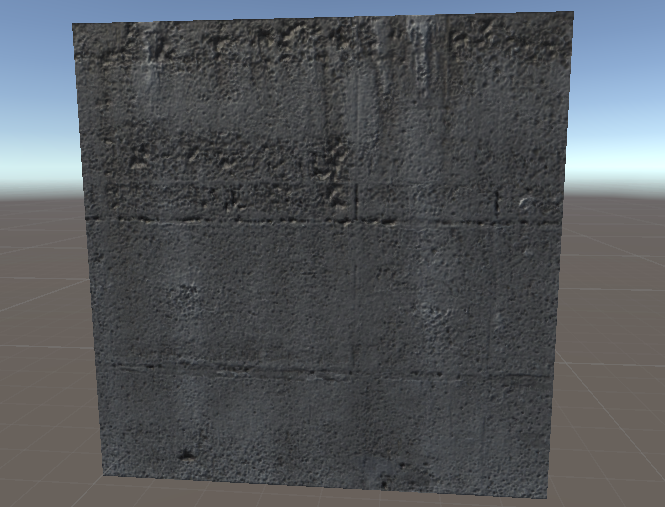
\includegraphics[scale = 0.85]{figures/Wall_tileable}
 	\caption{Przyk�ad tr�jwymiarowego modelu (�ciany) z jednokierunkowym tilingiem (�r�d�o: opracowanie w�asne)}
 \end{figure}
 \begin{figure}[!ht]
 	\centering
 	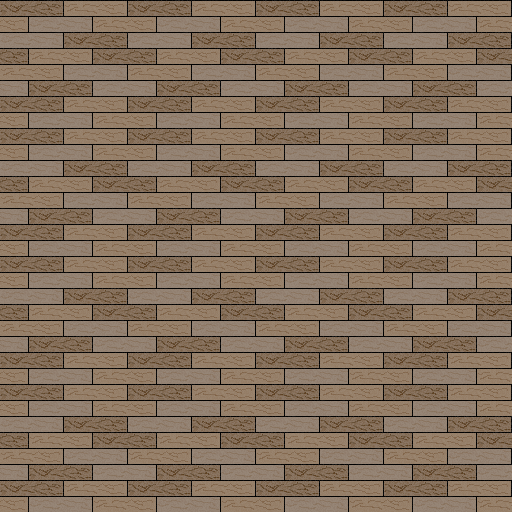
\includegraphics[scale = 0.65]{figures/Floor_wooden_2}
 	\caption{Przyk�ad tekstury (pod�ogi) z dwukierunkowym tilingiem (�r�d�o: opracowanie w�asne)}
 \end{figure}
 \newpage
 Mo�emy wyr�ni� dwa rodzaje zalet, kt�re niesie za sob� modularne podej�cie do procesu tworzenia poziom�w. Pierwsze z nich, to potencjalne korzy�ci dla samego procesu. Przyk�adem tutaj s� mi�dzy innymi:
 \begin{itemize}
 	\item W wi�kszo�ci przypadk�w pozwala na skr�cenie czasu potrzebnego na stworzenie poziomu, co pozwala na lepsze dopracowanie samych asset�w.
 	\item Mo�liwo�� wprowadzania poprawek na elementach ju� u�o�onych w docelowym silniku (pod warunkiem odpowiedniego zaprojektowania ich wcze�niej). Dzi�ki temu ludzie zajmuj�cy si� projektowaniem poziom�w do gier mog� rozpocz�� ich uk�adanie w silniku na bardzo wczesnym etapie produkcji. Przy odpowiednim ustawieniu punktu odniesienia w przestrzeni dla obiekt�w (ang. pivot point), obiekty mog� by� ustawione w docelowym po�o�eniu ju� na etapie wczesnych prototyp�w, by po jakim� czasie zosta� podmienione na finalne modele z teksturami bez dodatkowej ingerencji w pliki sceny.
 	\item Wielokrotne wykorzystanie tych samych modeli i tekstur wcale nie oznacza, �e poziomy w grze b�d� wygl�da�y na nudne i powtarzalne. Przy odpowiednim wykorzystaniu o�wietlenia, projektanci s� w stanie uzyskiwa� bardzo ciekawe efekty bez potrzeby tworzenia wielu asset�w. T� sytuacj� mo�emy zaobserwowa� na rysunku 2.3, gdzie por�wnano ten sam fragment sceny przy r�nych ustawieniach o�wietlenia.
  	\begin{figure}[!ht]
 		\centering
  		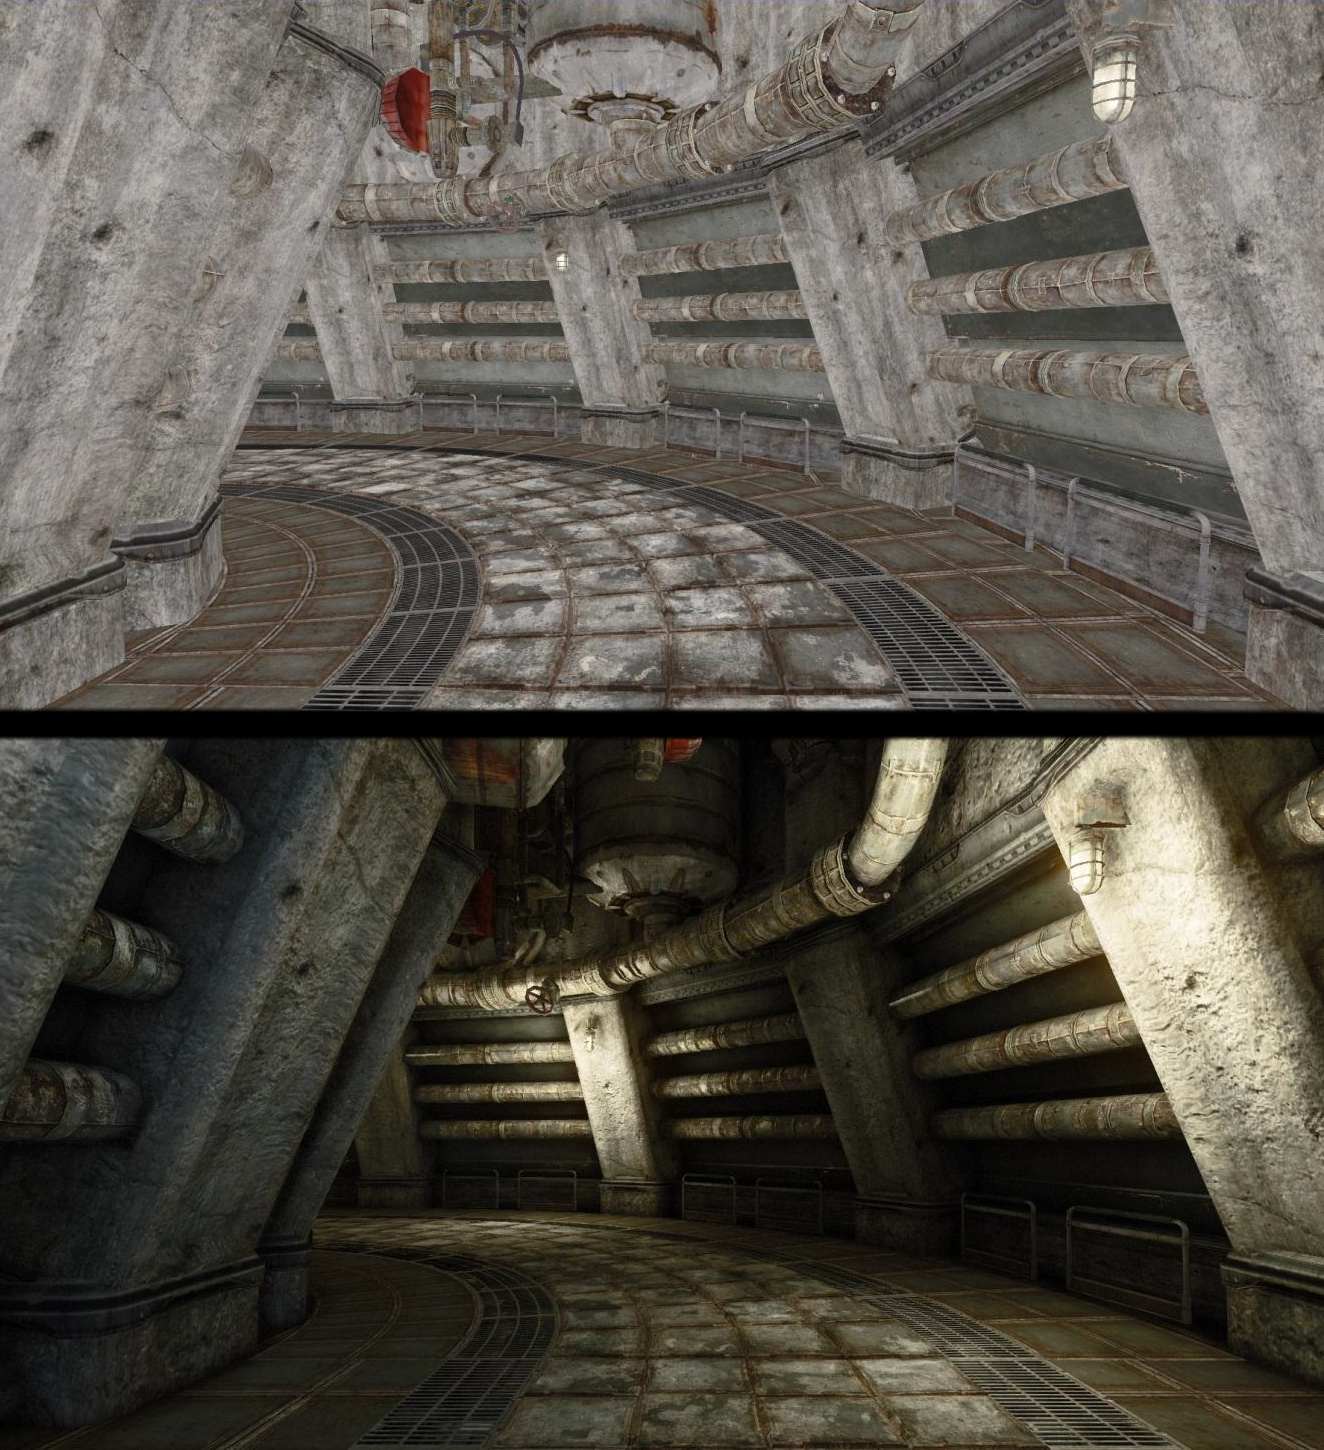
\includegraphics[scale = 0.20]{figures/Using_light_to_differ_assets}
  		\caption{Wykorzystanie o�wietlenia w celu ukrycia faktu wykorzystania niewielkiej ilo�ci modeli (�r�d�o: \cite{Investigation})}
 	\end{figure}
 \end{itemize}
 Dodatkowo, modularno�� pozwala na uzyskanie profit�w w kwestii wydajno�ci projektu. To w du�ej mierze z tego powodu zyska�a ona tak du�� popularno�� w�r�d tw�rc�w gier komputerowych, gdy� dla uzyskania maksymalnego komfortu rozgrywki nale�y jak najbardziej skr�ci� czas renderingu pojedynczej klatki obrazu. \newline
 
 Pierwszym z nich jest potencjalna oszcz�dno�� pami�ci karty graficznej. Jak to si� dzieje, �e mo�emy uzyska� taki efekt? Ot�, gdy chcemy by karta graficzna wyrenderowa�a nam klatk� obrazu, musimy najpierw zapewni� jej wszystkie potrzebne do tego dane. W�r�d nich znajdziemy chocia�by: orientacj� w przestrzeni obiekt�w (oraz wierzcho�k�w tych�e obiekt�w), koordynaty teksturowania, pozycje �wiate� oraz same tekstury. Wszystkie one musz� zosta� skopiowane do wewn�trznej pami�ci RAM karty graficznej. Je�li scena b�dzie sk�ada� si� z jednego, wielkiego modelu 3d, to b�dzie on musia� by� w ca�o�ci wczytany do pami�ci w celu jego dalszego wykorzystania w procesie renderingu. Stworzenie modu��w, kt�re nast�pnie zostaj� wielokrotnie instancjonowane w scenie pozwala na nieco inne potraktowanie danych przesy�anych do karty. Sam model zostaje skopiowany do pami�ci tylko raz, a dane dotycz�ce transformacji ka�dej z instancji (pozycji, rotacji i skali) s� przesy�ane niezale�nie od nich. Pozwala to na potencjalne oszcz�dno�ci w szczeg�lno�ci, gdy wielokrotnie wykorzystujemy dany modu�. \cite{GPUGems2} \newline
 
 Kolejnym argumentem przemawiaj�cym za stosowaniem modu��w jest zwi�kszenie przeno�no�ci i uniwersalno�ci samych asset�w. Analogicznie do poprzedniego przyk�adu - je�eli scena zosta�a stworzona jako jeden, wielki model to aby stworzy� nieco zmienion� jej wersj� nale�y skopiowa� ca�o��, wprowadzi� zmiany, a na koniec wyeksportowa� now� wersj� (r�wnie� jako jeden, du�y obiekt). Stwarza to przynajmniej trzy problemy:
 \begin{itemize}
 	\item Ka�da zmiana uk�adu sceny wymaga ingerencji w pliki �r�d�owe modeli 3d oraz ich ponowny eksport do silnika.
 	\item Nie jest mo�liwe ponowne wykorzystanie w prosty spos�b fragment�w sceny w innych projektach lub nawet w tym samym projekcie i kolejnych poziomach. Ka�dorazowe wykorzystanie element�w modelu wymaga ingerencji w pliki �r�d�owe oraz wyodr�bnienie ich od reszty siatki.
 	\item Wspomniana ju� wcze�niej pami�� karty graficznej zostaje niepotrzebnie zapisana nadmiarowymi danymi, kt�re mog�yby zosta� zast�pione instancjonowaniem.
 \end{itemize}
 Wszystkie trzy problemy eliminuje zaprojektowanie i stworzenie modu��w, z kt�rych dopiero p�niej s� budowane docelowe poziomy w zale�no�ci od aktualnych potrzeb projektanta. Dodatkowo pozwala r�wnie� na do�� wygodne oddzielenie pracy projektanta poziom�w od artysty tworz�cego modele i tekstury.
\begin{figure}[!ht]
	\centering
	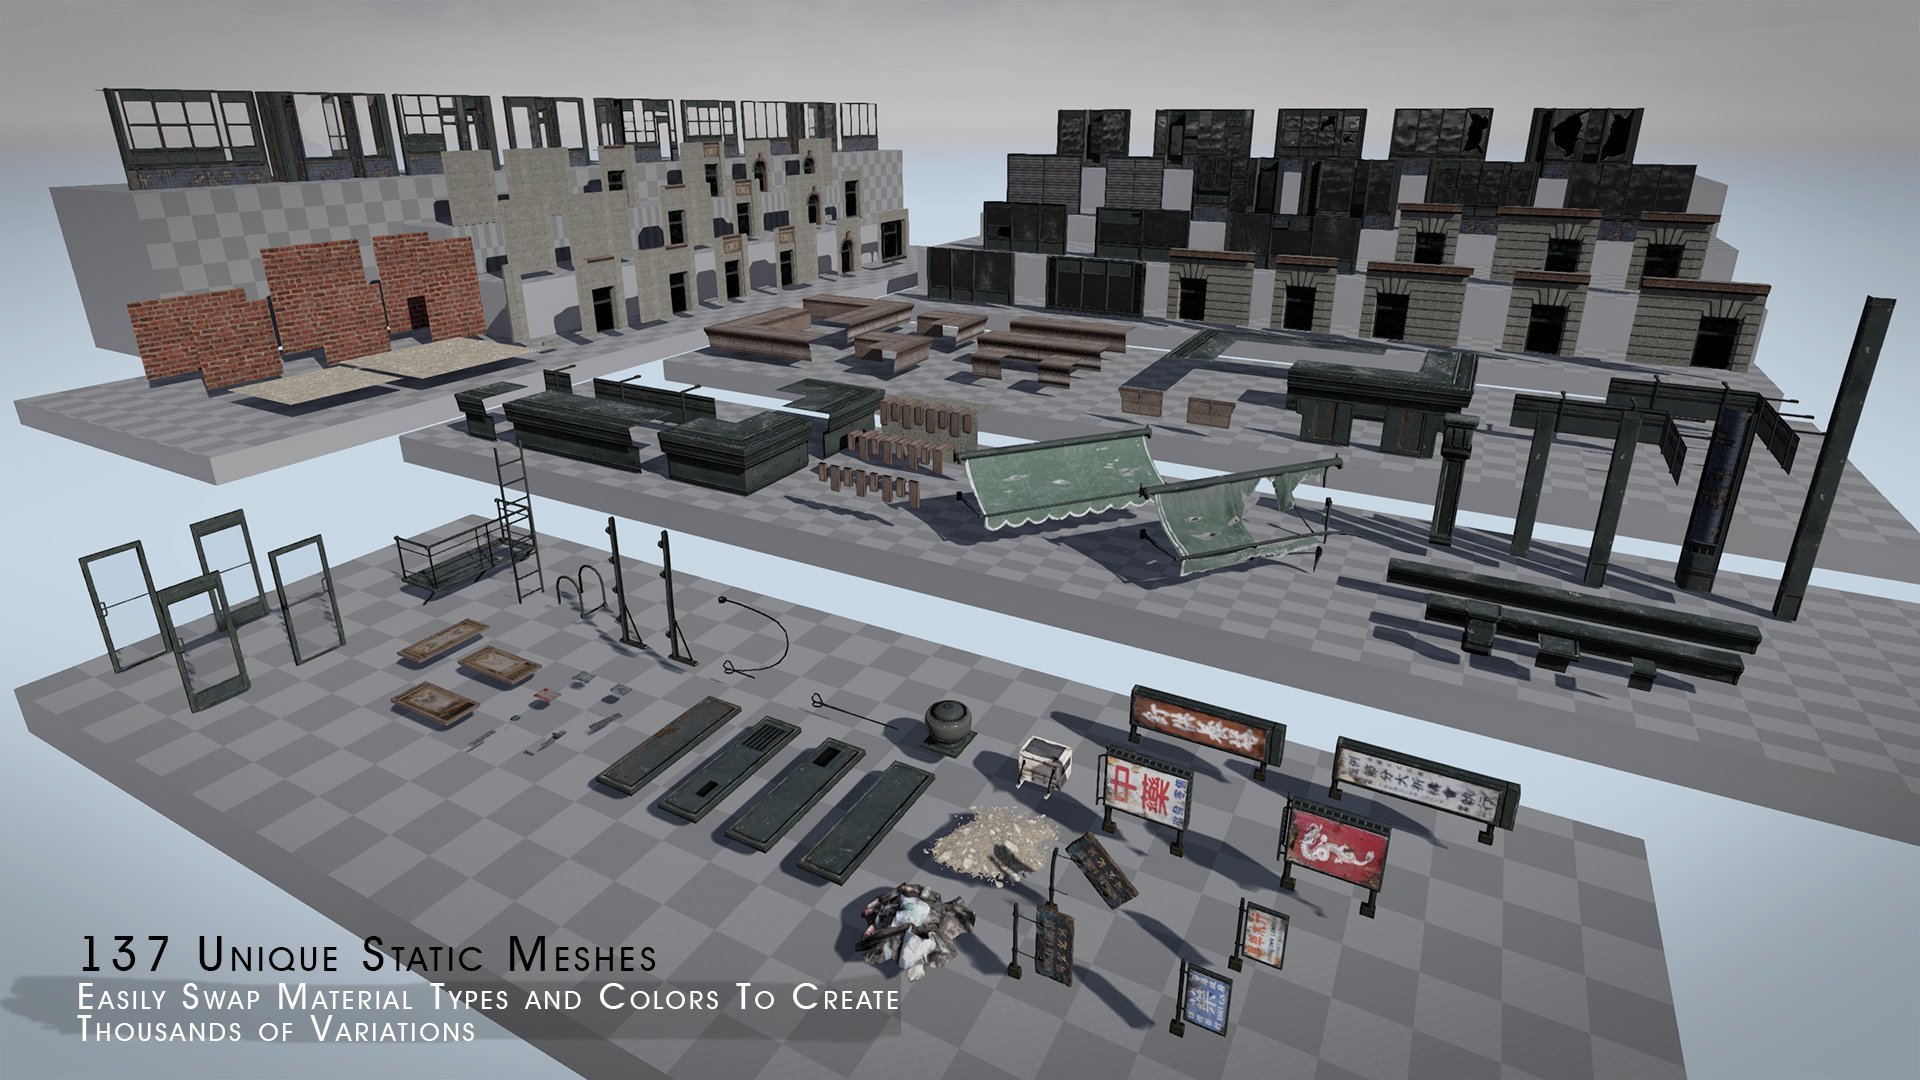
\includegraphics[scale = 0.20]{figures/AssetsPack}
	\caption{Przyk�adowa paczka modularnych modeli (�r�d�o: \cite{ModularPack})}
\end{figure}
\section{Atlasowanie}
Atlasowanie jest procesem maj�cym na celu zebranie wielu niekoniecznie powi�zanych ze sob� asset�w w jedn� ca�o�� oraz przechowywanie ich w jednym, du�ym pliku. Mo�liwe jest stosowanie go zar�wno w odniesieniu do siatek wielok�towych, jak i tekstur - cho� z regu�y cz�ciej spotykan� praktyk� jest wykorzystywanie atlas�w tekstur.\newline 

Mimo pewnych problem�w, jakie niesie za sob� stosowanie tej techniki podczas pracy, wielu tw�rc�w stosuje j� w swoich projektach. Jest tak g��wnie dlatego, �e daje ona sporo korzy�ci w kwestii potencjalnej wydajno�ci projektu. S� to przede wszystkim:
\begin{itemize}
	\item \textbf{Potencjalna oszcz�dno�� pami�ci operacyjnej}
	\item \textbf{Mniej draw calli podczas renderowania sceny}
	\item \textbf{�atwiejszy dost�p do wielu tekstur jednocze�nie}
\end{itemize}

Jak ju� zosta�o wspomniane wcze�niej, atlasowanie mo�na stosowa� zar�wno dla modeli, jak i tekstur. Poni�ej opisano w jaki spos�b post�puje si� zar�wno w jednym, jak i drugim przypadku:
\begin{itemize}
	\item \textbf{Atlasy tekstur}
	\item \textbf{Atlasy modeli}
\end{itemize}

Wykorzystywanie atlas�w wi��e si� jednak z pewnymi utrudnieniami, z kt�rymi nale�y liczy� si� podczas procesu produkcji.
\begin{itemize}
	\item \textbf{Du�y rozmiar plik�w na repozytorium} - 
	\item \textbf{Dodatkowe nak�ady pracy przy r�cznym uk�adaniu atlas�w} - 
\end{itemize}

\section{Wykorzystywanie mo�liwo�ci u�ywanego silnika}
R�wnie wa�ne, jak stosowanie uniwersalnych technik optymalizacji, jest zapoznanie si� z mo�liwo�ciami oferowanymi przez wybran� technologi�, na kt�rej tworzony jest projekt gry. Pozwala to nie tylko na uzyskanie lepszych wynik�w w kwestii wydajno�ci, ale tak�e na poprawienie jako�ci samej grafiki wy�wietlanej na ekranie gracza. Poniewa� docelowym silnikiem, na kt�rej realizowano cz�� praktyczn� tej pracy jest \textit{Unreal Engine 4}, to w tej cz�ci przybli�one zostan� cechy charakterystyczne dla tej technologii:
\begin{itemize}
	\item \textbf{Physically based rendering} - 
	\item \textbf{Maskowanie} - 
\end{itemize}

% !TeX encoding = windows-1250

\chapter{Opis procesu}
\label{t:description}
Rozdzia� ma za zadanie ukazanie procesu tworzenia poziomu od etapu wczesnego planowania a� do finalnej sceny z o�wietleniem. Ka�dy etap zosta� pokr�tce opisany: dlaczego si� go stosuje i jak mo�na podej�� do niego w optymalny spos�b. Przyk�ady oparte s� w g��wnej mierze o do�wiadczenie tw�rc�w zajmuj�cych si� tym od wielu lat - takimi, jak chocia�by Epic Games czy Bethesda Softworks - kt�rzy swoimi spostrze�eniami dziel� si� na wszelakiego rodzaju konferencjach i w publikowanych artyku�ach.
\section{Podzia� obrazka na modularne tekstury i modele}
Po obraniu wizji artystycznej narzuconej przez grafika koncepcyjnego zaczynaj� si� pierwsze prace projektowe maj�ce na celu wyeliminowanie jak najwi�kszej liczby b��d�w na p�niejszych etapach produkcji. Gdy projektant dostaje do dyspozycji grafik� koncepcyjn� lokacji, cz�sto pierwszym krokiem jest odnalezienie na niej potencjalnych modu��w oraz wyr�nienie ich. Zwykle robi si� to dwukrotnie: pierwszy podzia� dokonywany jest z uwzgl�dnieniem potencjalnych kandydat�w na tr�jwymiarowe siatki wykorzystane jako modu�y, natomiast drugi bierze pod uwag� jak najoptymalniejsze wykorzystanie tekstur w procesie. Proces ten cz�sto zwany jest ''scene breakout'' - czyli w lu�nym t�umaczeniu rozbicie sceny. \newline
Podczas wyodr�bniania element�w nale�y szuka� modu��w w taki spos�b, aby wydoby� jak najmniejsze, mo�liwe do samodzielnego wykorzystania elementy (np. fragment kolumny mo�na wykorzysta� r�wnie� jako podest lub rodzaj o�tarza), lub takie, kt�re same w sobie nie s� zwykle wykorzystywane niezale�nie, ale cz�st� praktyk� b�dzie ich podmiana na inne warianty kolorystyczne lub kszta�ty (tutaj dobrym przyk�adem s� chocia�by okna lub drzwi, kt�re warto wyodr�bni� od modu��w �cian).\newline
Rozbijanie sceny ma na celu wst�pne oszacowanie liczby wymaganych do stworzenia asset�w oraz da� tw�rcom pogl�d na to, jak mog� one wygl�da�. Dzi�ki temu, �e nie wymaga zbyt wielkich nak�ad�w czasowych, jest cz�sto stosowan� technik� przez tw�rc�w grafiki tr�jwymiarowej w grach komputerowych. Praktykuj� go chocia�by u�ytkownicy bran�owego forum polycount.com podczas comiesi�cznego \textit{Monthly Community Noob Challenge}. Przyk�ad przeprowadzenia scene breakoutu widoczny jest na rysunku 3.1.
\begin{figure}[!ht]
	\centering
	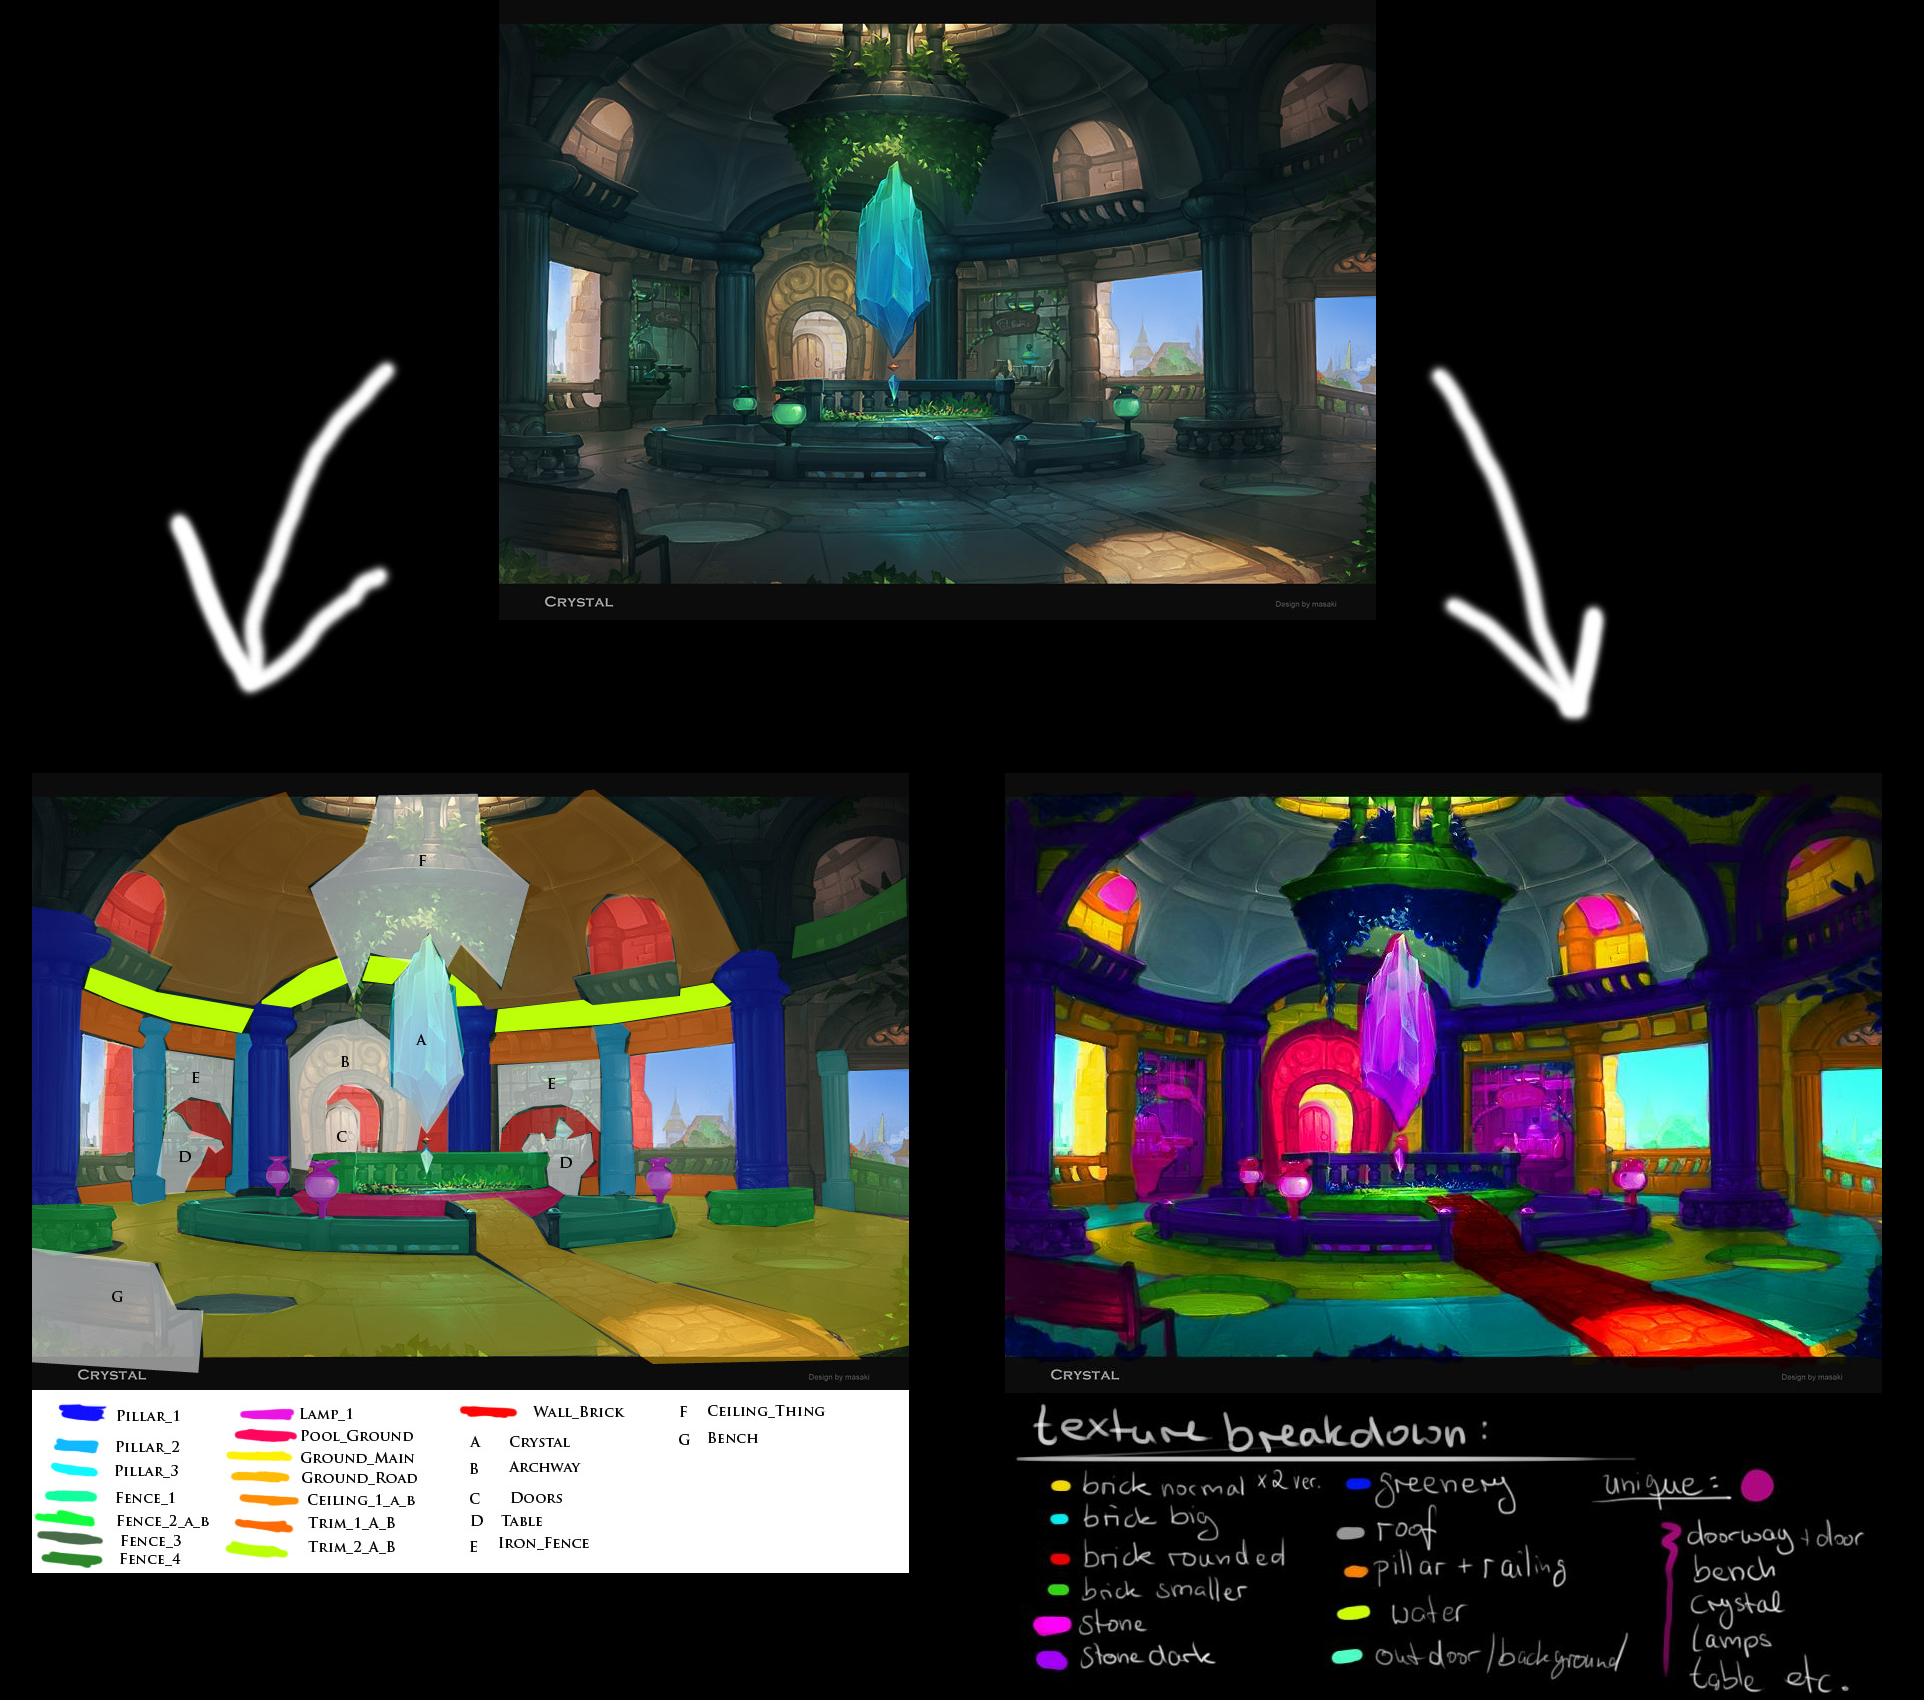
\includegraphics[scale = 0.24]{figures/Scene_breakdown}
	\caption{Przyk�adowy podzia� sceny z uwzgl�dnieniem modeli (po lewej) oraz tekstur (po prawej) (�r�d�o: \cite{NoobChallengeAugust2013})}
\end{figure}
\section{Tworzenie dokumentacji projektowej}
Etap pisania dokumentacji projektowej jest szczeg�lnie wa�ny w przypadku, gdy nad tworzeniem poziom�w pracuje kilka lub nawet kilkana�cie os�b. Pozwala ona na ujednolicenie samego procesu w�r�d wszystkich tw�rc�w, minimalizuje ryzyko zdublowania pracy przez kilka os�b (na przyk�ad wykonania tego samego modelu przez dw�ch artyst�w 3d), a tak�e pozwala jasno okre�li� obrany kierunek artystyczny, kt�rego maj� trzyma� si� wszyscy bior�cy udzia� w procesie.\newline
Podczas tworzenia takiej dokumentacji warto wzi�� pod uwag� takie elementy, jak chocia�by:
\begin{description}
	\item[Tworzenie listy asset�w] \hfill \\
	Po wst�pnym wydzieleniu asset�w na grafikach koncepcyjnych warto wypisa� szczeg�ow� list� wszystkich modeli oraz tekstur, kt�re zostan� zamieszczone w finalnej paczce. W przypadku siatek 3d warto r�wnie� zapisa� wymagany rozmiar w przestrzeni oraz liczb� kierunk�w tilingu (1, 2 lub jego brak). Podczas wpisywania tekstur, opr�cz wymienionych ju� aspekt�w, mo�na zwr�ci� dodatkow� uwag� na ich umiejscowienie w atlasie - w kt�rym z atlas�w (je�li jest ich kilka) oraz w kt�rym jego miejscu ma si� ona znajdowa�. \newline
	Taka lista mo�e nast�pnie zosta� opublikowana zespo�owi projektant�w i grafik�w w postaci zada� do wykonania lub nawet zwyk�ego, wsp�dzielonego w chmurze dokumentu.
	\item[Jednostki miary w silniku oraz grid] \hfill \\
	Bardzo wa�n� kwesti�, kt�r� nale�y rozpatrze� jest dostosowanie ustawie� programu do edycji modeli 3d do wymaga� stawianych przez silnik gry. Najwi�kszym problemem, kt�ry koniecznie trzeba rozpatrze� jest dob�r jednostek stosowanych w docelowej technologii. Najwi�ksz� konsekwencj� id�c� za tym wyborem jest zmieniaj�ca si� skala siatki wed�ug kt�rej ustawiane s� docelowe modele (ang. grid). Uk�adanie modeli za pomoc� gridu jest jedn� z najwi�kszych zalet modu�owego tworzenia poziom�w. Pozwala ona znacznie skr�ci� czas pracy projektant�w, gdy� usuwa z procesu konieczno�� obliczania koordynat�w ka�dego obiektu i pozwala je ustawia� sugeruj�c si� liniami wy�ej wspomnianej siatki. Obecnie najpopularniejsze s� dwa rozwi�zania stosowane przez tw�rc�w. Poni�ej je przedstawi�, a tak�e spr�buj� przybli�y� potencjalne zalety i wady obu podej��:
	\begin{itemize}
		\item \textbf{System metryczny} - stosowany chocia�by w \textit{Unreal Engine 4}. Podstawow� jednostk� miary jest zwykle centymetr, a kolejne elementy siatki uk�adane s� co X centymetr�w - gdzie X jest dowoln� liczb� obran� przez u�ytkownika. Z regu�y przyjmuje si� �e przy takim systemie posta� ma oko�o 180 jednostek wzrostu. Do zalet takiego podej�cia nale�y na pewno jego intuicyjno�� w odniesieniu do pomiar�w czynionych w �wiecie rzeczywistym - mo�na bezproblemowo odwzorowywa� wymiary rzeczywistych obiekt�w bez dodatkowych oblicze�. Za wad� mo�na uzna� potencjalne problemy podczas skalowania obiektu (zw�aszcza, gdy jest on zmniejszany), gdy� w przypadku modu��w zwykle stosuje si� zasad�, �e obiekty skalowane s� o kolejne pot�gi liczby 2. \cite{CreatingModularGameArt}
		\item \textbf{System oparty o pot�gi liczby 2} - wykorzystywany w \textit{Unreal Engine 3}. W przeciwie�stwie do poprzedniego systemu u�ytkownik ma mniejszy wyb�r je�li chodzi o ustawienia siatki. Zwykle uk�adana jest co $2^n$ jednostek silnika (n obierane jest przez u�ytkownika). Posta� przy takim podej�ciu ma oko�o 96 jednostek wysoko�ci. System eliminuje problem podczas skalowania obiekt�w w d� (jest tak poniewa� powsta� on na podstawie liczby 2), jednak mo�e sprawia� problemy przy przeliczaniu wymiar�w (zw�aszcza podczas modelowania obiekt�w znanych ze �wiata rzeczywistego). \cite{CreatingModularGameArt}
	\end{itemize}
	Ujednolicenie ustawie� programu w kt�rym tworzone s� modele jest kluczowe dla dalszej bezproblemowej eksploatacji wytworzonych asset�w. \newline
	Niekt�rzy tw�rcy kreuj� jeszcze inne systemy miar w swoich silnikach. Dobrym przyk�adem mo�e by� tu Bethesda - w silniku rozwijanym przez t� firm� posta� ma oko�o 128 ($2^7$) jednostek wzrostu. Mo�emy to zobaczy� na udost�pnionej grafice (Rysunek 3.2).
	\begin{figure}[!ht]
		\centering
		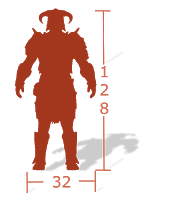
\includegraphics[scale = 0.84]{figures/Unit_scale}
		\caption{Posta� w silniku firmy Bethesda Softworks (�r�d�o: \cite{Skyrim})}
	\end{figure}
	\item[Parametry eksportu] \hfill \\ 
	Podobnie jak z ustawieniem jednostek oraz rozmieszczeniem gridu - parametry eksportu modeli do danego silnika maj� bardzo du�e znaczenie. Dobr� konfiguracj� samego programu mo�na popsu� z�ymi ustawieniami eksportera. W dokumentacji warto uj�� kilka kwestii (zak�adaj�c, �e eksportujemy pliki do formatu .fbx):
	\begin{itemize}
		\item Jakiej skali chcemy u�ywa� przy eksporcie. Tutaj zwykle ustawiamy to w taki spos�b, aby wynosi�a ona dok�adnie 1.
		\item Jakie elementy sceny maj� znale�� si� w pliku. To pozwala unikn�� przypadkowego wyeksportowania element�w, kt�re nie powinny si� tam znale��. W�r�d nich mo�na wymieni� chocia�by: siatki wielok�towe, ko�ci i animacje, kamery, �wiat�a, czy te� elementy pomocnicze.
		\item Jakie parametry samych modeli maj� zosta� umieszczone. Niekt�re silniki potrzebuj� �ci�le okre�lonych ustawie� eksportu siatki. Tutaj dobrym przyk�adem jest \textit{Unreal Engine 4}, kt�ry wymaga dodatkowego zamieszczenia grup wyg�adzania w celu poprawnego importu siatki.
	\end{itemize}
	\begin{figure}[!ht]
		\centering
		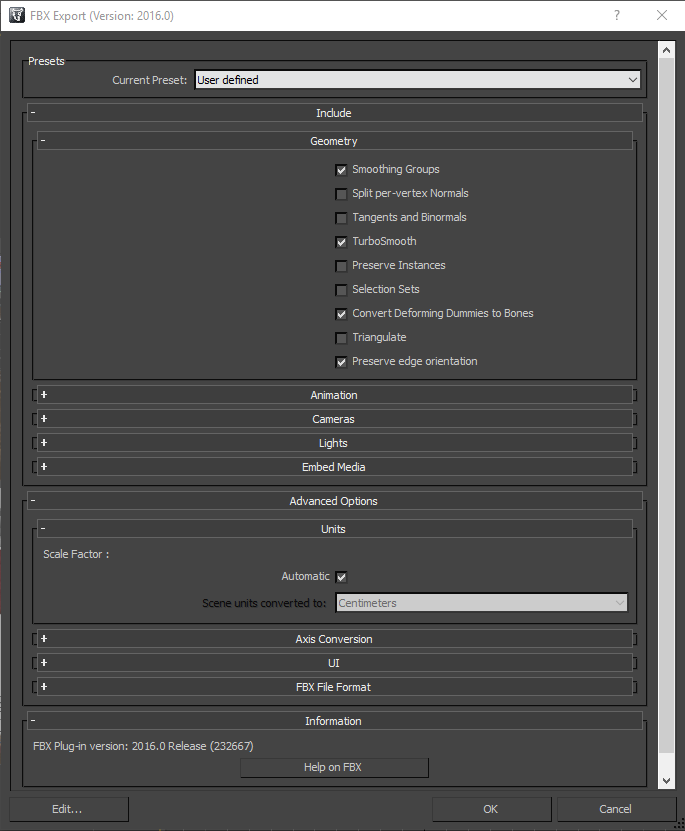
\includegraphics[scale = 0.70]{figures/Export_parameters}
		\caption{Ustawienia eksportu dla statycznych modeli w programie \textit{Autodesk 3ds Max} (�r�d�o: opracowanie w�asne)}
	\end{figure}
	\item[Nazewnictwo] \hfill \\
	Konwencje nazewnictwa s� kwesti� z pozoru niewiele znacz�c�. Jednak podczas tworzenia poziom�w z modu��w projektanci mog� bardzo szybko pogubi� si� w nat�oku asset�w, kt�re s� nazywane w niejasny spos�b. Dlatego te� stosowane s� �cis�e zasady nazewnictwa. Pozwalaj� one na szybkie odnalezienie przeznaczenia danego modelu bez wcze�niejszego ustawiania go w scenie, a czasami nawet bez u�ywania podgl�du. Przyk�adem implementacji wewn�trznej konwencji nazewnictwa mo�e by� ta stosowana przez firm� Bethesda Softworks. Przeanalizujmy asset, kt�rego nazwa brzmi: ''UtlBayCorInMidPRTT01L01'': \cite{Skyrim}
	\begin{itemize}
		\item \textbf{Utl} - oznacza, �e jest on cz�ci� pakietu ''Utility''
		\item \textbf{Bay} - oznacza, �e jest on cz�ci� pakietu ''Bay'' (wchodzi on w sk�ad ''Utility'')
		\item \textbf{Cor} - jest to fragment oznaczaj�cy, �e mamy do czynienia z elementem naro�nym (ang. corner oznacza naro�nik)
		\item \textbf{In} - oznacza, �e jest to naro�nik wewn�trzny (zamiast tego, mogliby�my tu znale�� ''Out'', kt�re oznacza�oby wygi�cie w przeciwnym kierunku)
		\item \textbf{Mid} - okre�la kierunek tilingu. W tym wypadku element mo�emy dopasowywa� wertykalnie
		\item \textbf{PRTT01} - tego fragmentu tw�rca artyku�u nie potrafi� rozszyfrowa�
		\item \textbf{L} - skr�cone ''Left''. U�ywane przez tw�rc�w do rozr�nienia modeli odbitych lustrzanie
		\item \textbf{01} - pozwala rozr�nia� r�ne wersje wizualne danego assetu		
	\end{itemize}
	Je�li osoba tworz�ca modele stosuje si� do podobnego systemu, ju� po samych nazwach asset�w da si� (przynajmniej w przybli�eniu) okre�li� potencjalne ich zastosowanie. Kluczem jest tutaj dyscyplina w trzymaniu si� konwencji.
	\begin{figure}[!ht]
		\centering
		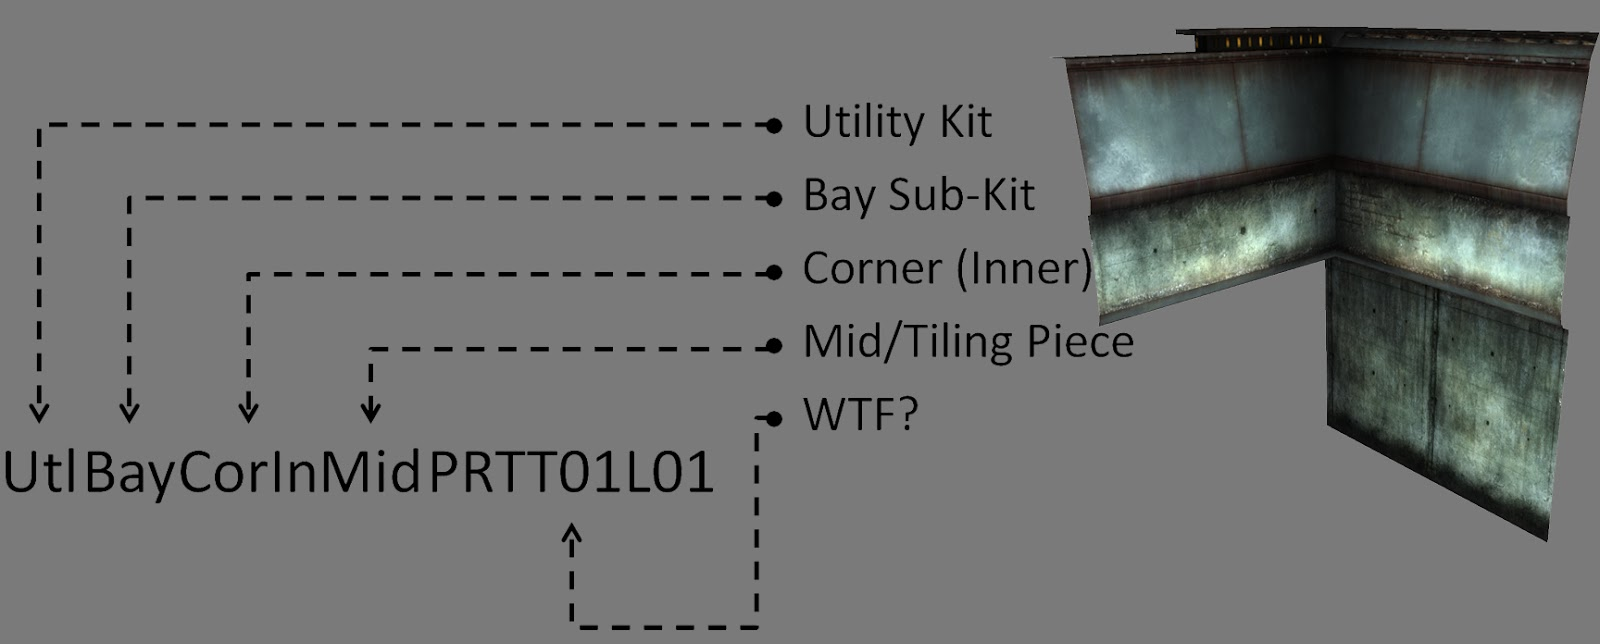
\includegraphics[scale = 0.20]{figures/Skyrim_names}
		\caption{Nazewnictwo stosowane w firmie Bethesda Softworks (�r�d�o: \cite{Skyrim})}
	\end{figure}
	\item[Referencje] \hfill \\
	Zbieranie obraz�w referencyjnych jest wa�nym etapem preprodukcji ka�dego poziomu. Bez nich bardzo trudno jest stworzy� co�, co wygl�da realistycznie, autentycznie oraz jest wysokiej jako�ci. \cite{UltimateLevelDesign} Ludzki umys� nie radzi sobie najlepiej z zapami�tywaniem detali, dlatego warto gromadzi� rysunki, kt�re pozwalaj� je odtworzy� w p�niejszym etapie. \newline
	Referencje mo�emy podzieli� na kilka kategorii w zale�no�ci od ich docelowego zastosowania. Wyr�niamy referencje:
	\begin{itemize}
		\item \textbf{architektoniczne} - zawieraj� w sobie odno�niki do styl�w architektonicznych, w kt�rych maj� by� wykonane modele i tekstury - w szczeg�lno�ci budowli.
		\item \textbf{�rodowiskowe} - daj� pogl�d na �rodowisko w jakim b�dzie porusza� si� potencjalny gracz
		\item \textbf{o�wietleniowe} - ukazuj� jak musz� zosta� o�wietlone poziomy w celu uzyskania odpowiedniego klimatu.
		\item \textbf{skupione na detalach} - daj� wgl�d w ewentualne detale, kt�re mog� zosta� umieszczone na modelach
		\item \textbf{inspiracje} - dodatkowe obrazy lu�no zwi�zane z tematyk� pracy. Maj� na celu rozszerzy� perspektyw� tw�rcy i dostarczy� mu dodatkowych inspiracji podczas tworzenia grafik
	\end{itemize}
	\begin{figure}[!ht]
		\centering
		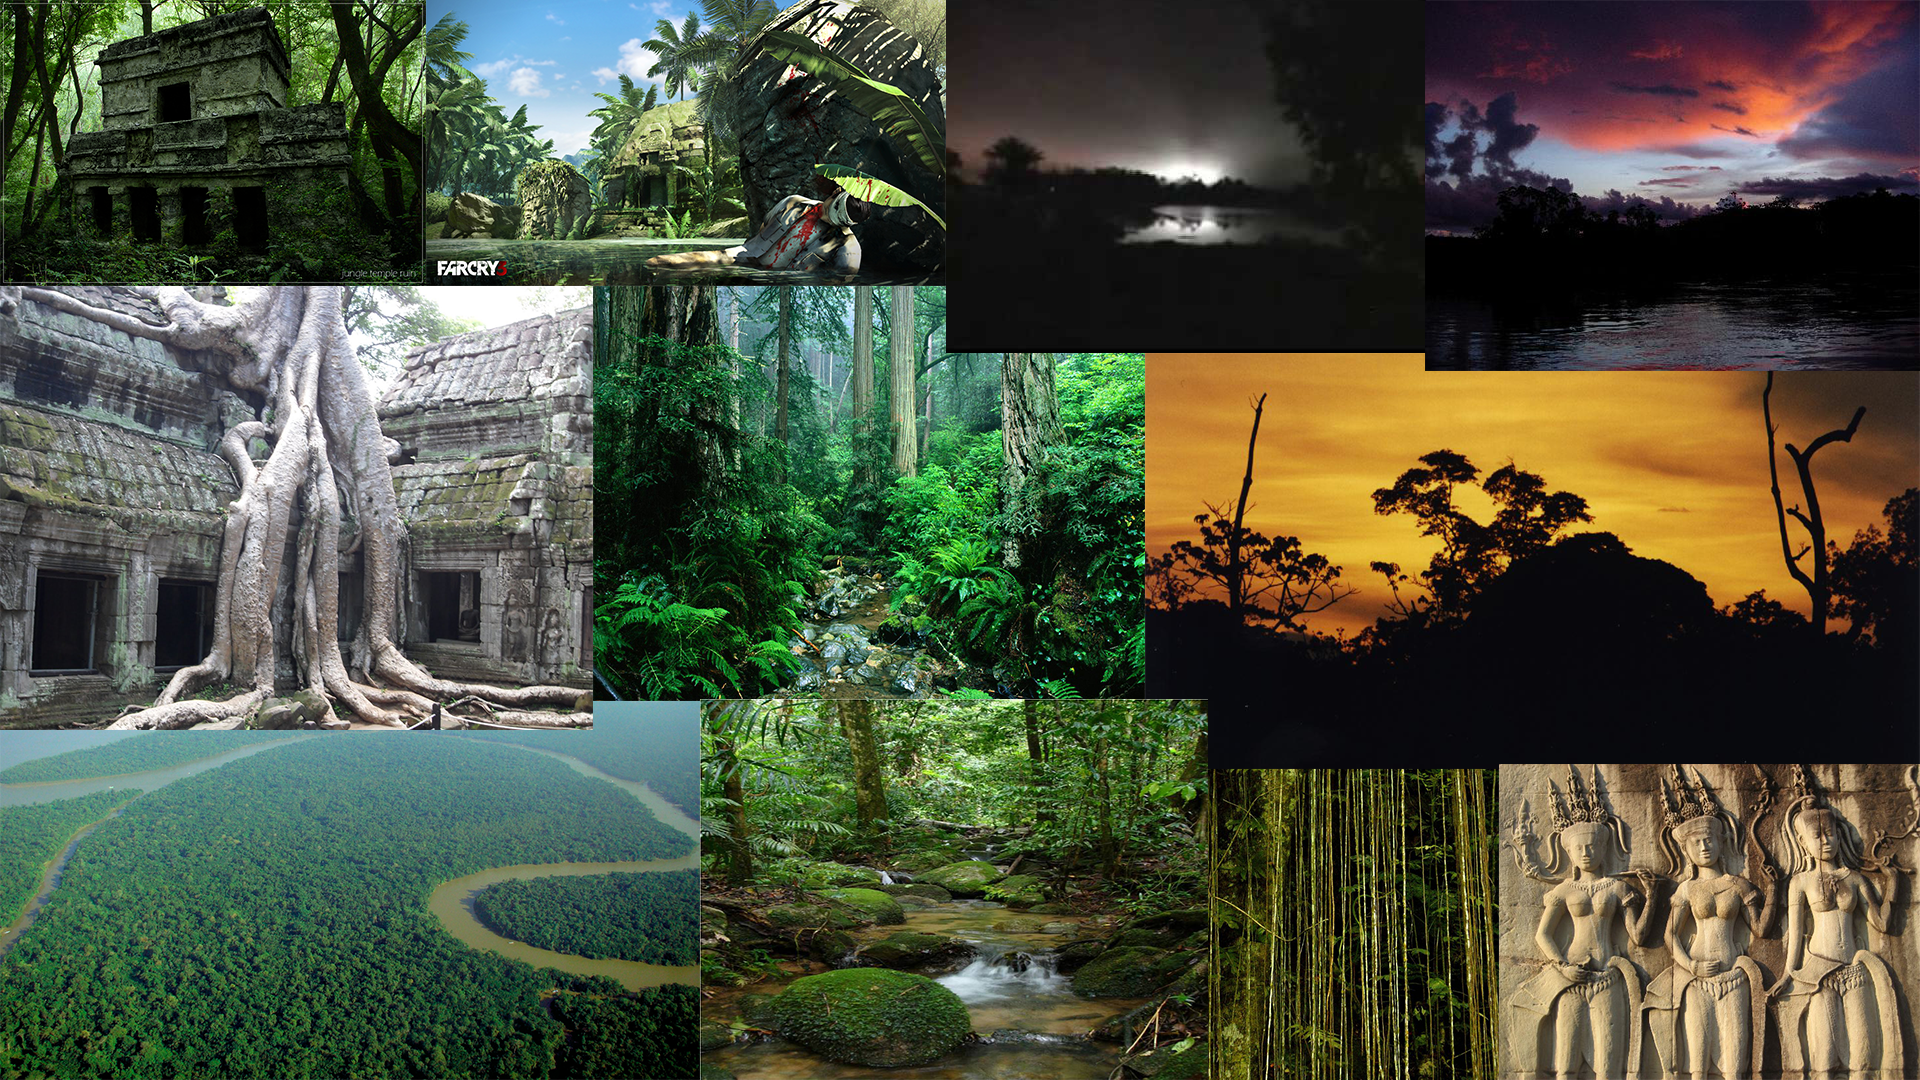
\includegraphics[scale = 0.20]{figures/References}
		\caption{Zbi�r referencji (tzw. mudboard) (�r�d�o: opracowanie w�asne)}
	\end{figure}
\end{description}
Tak opracowana dokumentacja projektowa pozwala na wyeliminowanie wielu problem�w, kt�re mog�yby powsta� podczas pracy w kilkuosobowym zespole (zw�aszcza na linii graficy - projektanci). Dlatego warto po�wi�ci� czas jeszcze podczas fazy preprodukcji, aby p�niej w du�o prostszy spos�b m�c kontrolowa� prac� zespo�u tw�rc�w.
\section{Tworzenie tymczasowych wersji asset�w oraz testy}
	Ta faza ma na celu szybkie stworzenie prototyp�w asset�w, kt�re b�d� w pe�ni funkcjonalne, jednak jeszcze dalekie od finalnej wersji wizualnej. Pozwala to sprawdzi�, czy koncepcja tworzenia modeli jest s�uszna i czy nie pomini�to w procesie jakiego� istotnego faktu. Po przej�ciu przez faz� pierwszych test�w, modele mog� by� ustawiane na finalnych pozycjach w poziomie. G��wnym wymaganiem, jakie musz� spe�ni�, aby to si� sta�o jest odpowiednie ustawienie pivot�w.
	
	
	\textbf{Pivoty} \newline
	Pivoty s� punktami wzgl�dem kt�rych dokonuje si� wszelkich transformacji lokalnych na tr�jwymiarowej siatce. Dlatego ich umiejscowienie jest wa�ne dla p�niejszych ewentualnych modyfikacji modelu.  Ma do szczeg�lnie du�e znaczenie podczas skalowania i obracania obiekt�w. Etap prototypowania jest doskona�� okazj� do przetestowania s�uszno�ci ich umiejscowienia. Paul Mader w swoim artykule na temat tworzenia modularnych asset�w wymienia 5 aspekt�w, kt�re nale�y wzi�� pod uwag� podczas wybierania tych punkt�w. Ich waga ro�nie wraz z pozycj�: \cite{CreatingModularGameArt}
	\begin{enumerate}
		\item \textbf{Punkt centralny} - u�ywany w modelach od kt�rych nie wymaga si� dok�adnego spasowania mi�dzy elementami. Przyk�adem mog� by� tu chocia�by kamienie.
		\item \textbf{Symetria} - w symetrycznych obiektach nale�y obiera� punkt znajduj�cy si� na osi symetrii (dodatkowo kieruj�c si� poprzednim punktem mo�na umie�ci� go w �rodku masy).
		\item \textbf{U�o�enie w �rodowisku} - obiekty, kt�re b�d� po�o�one w �wiecie w okre�lony spos�b, powinny mie� ustawiony punkt pivotu tak, aby jak najbardziej u�atwi� ich umiejscowienie (na przyk�ad u skrzy� powinna to by� ich dolna cz��, co u�atwi uk�adanie na pod�odze).
		\item \textbf{Tiling} - siatki wykorzystuj�ce tiling powinny mie� umieszczony punkt pivotu tak, aby da�o si� bezproblemowo ��czy� je z kolejnymi modu�ami.
		\item \textbf{O� obrotu} - najwa�niejszym aspektem, kt�ry powinien by� pod uwag� jest punkt obrotu. Ma to szczeg�lnie du�e znaczenie w przypadku modeli, kt�re maj� tworzy� �rodowisko na planie okr�gu. Odpowiednie dobranie pivotu w tym przypadku pozwala unikn�� problem�w z niedopasowanymi siatkami po obr�ceniu. 
	\end{enumerate}
	Przyk�ady umiejscowienia pivot�w z powy�szej listy znajdziemy na rysunku 3.6.
	\begin{figure}[!ht]
		\centering
		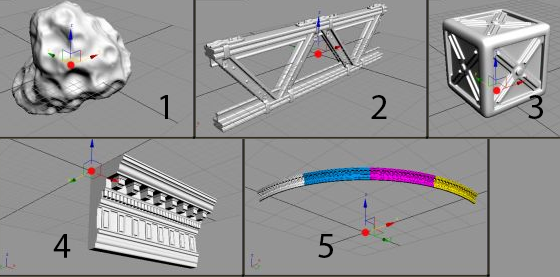
\includegraphics[scale = 0.83]{figures/Pivots}
		\caption{R�ne rodzaje umiejscowienia pivot�w (�r�d�o: \cite{CreatingModularGameArt})}
	\end{figure}	
	\begin{figure}[!ht]
		\centering
		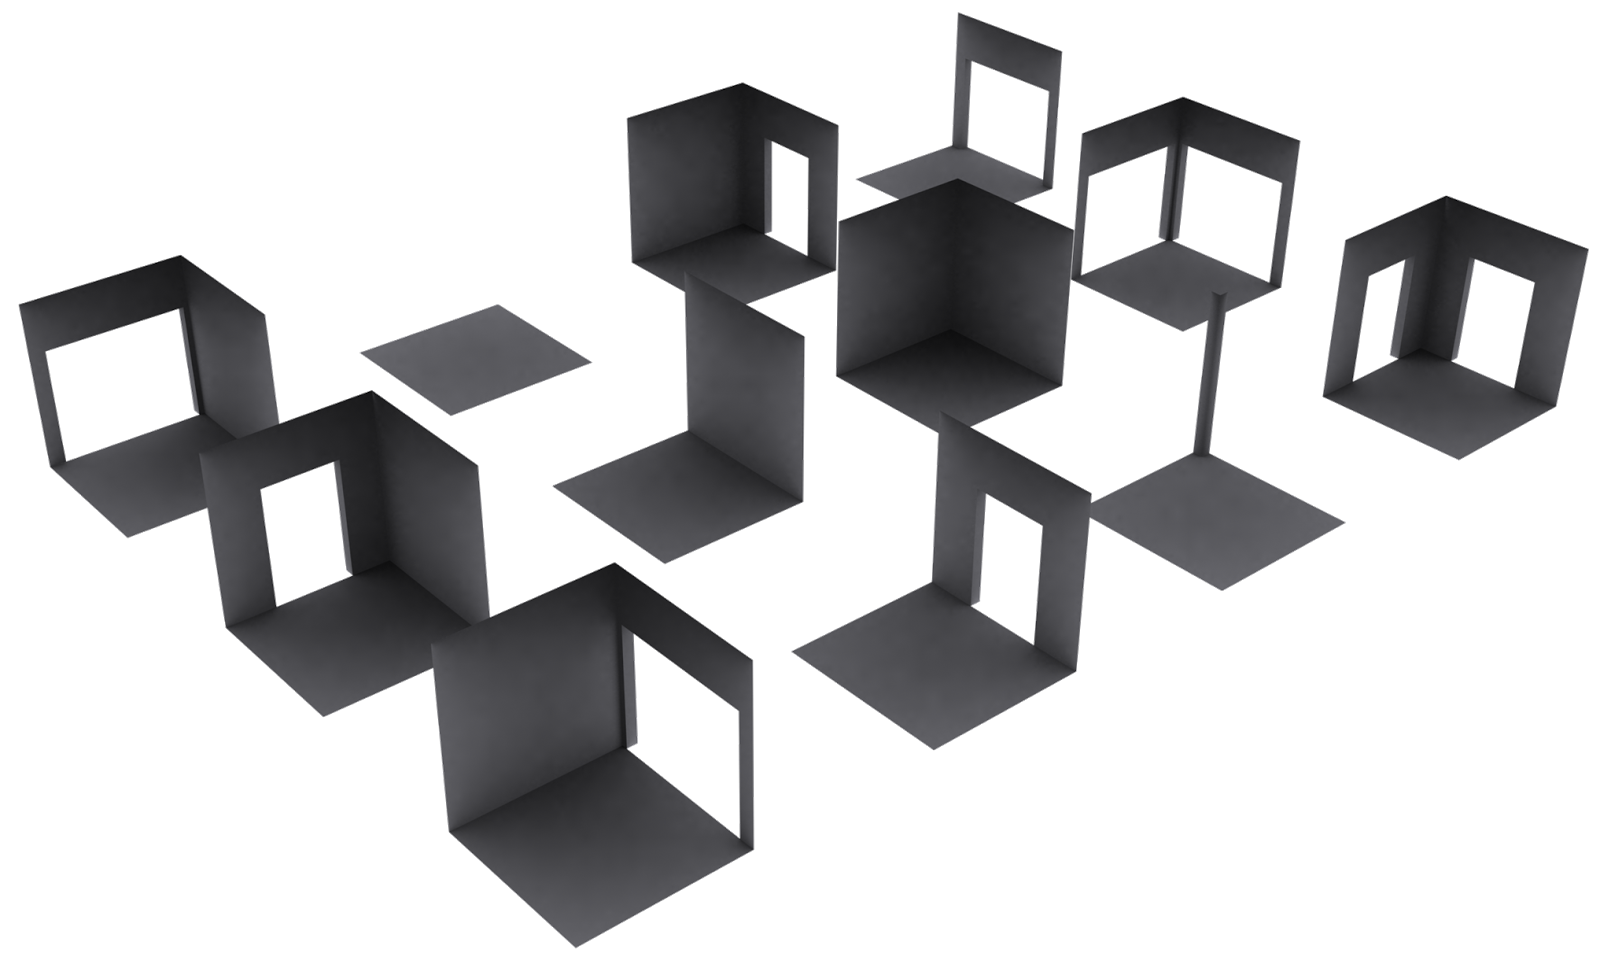
\includegraphics[scale = 0.23]{figures/Alpha_models}
		\caption{Paczka modeli w fazie prototypu (�r�d�o: \cite{Skyrim})}
	\end{figure}	
\section{Tworzenie finalnych wersji modeli i tekstur}
Po przej�ciu przez faz� prototypu proces tw�rczy mo�e przej�� w dwie niezale�ne od siebie �cie�ki. Pierwsz� z nich jest tworzenie contentu graficznego, czyli dodawanie szczeg��w graficznych, mapowanie koordynat�w UV oraz teksturowanie. Druga z nich, to uk�adanie sceny w silniku graficznym przez projektanta. Dzi�ki wcze�niej poczynionym planom oraz testom z do�� du�� pewno�ci� mo�na stwierdzi�, �e po podmianie tymczasowych modeli na ich finalne wersje poziom b�dzie wygl�da� tak, jak zaplanowa� sobie tego level designer. Zwykle ten etap jest najd�u�szy spo�r�d ca�ego procesu tworzenia paczki asset�w. W przypadku du�ych projekt�w AAA mo�e on trwa� nawet kilka miesi�cy \cite{Skyrim}.\newline
Podczas tworzenia finalnych modeli i tekstur nale�y r�wnie� uwa�a� na potencjalny problem wygl�du poziomu. Modularno�� ma to do siebie, �e �atwo mo�na wprowadzi� du�� monotoni� w scenie.\cite{UDNLevelDesign} Mo�na to prze�ama� poprzez tworzenie coraz wi�kszej liczby wariant�w kolorystycznych samych asset�w, co sprawia, �e �atwiej pogubi� si� w nat�oku dost�pnych mo�liwo�ci. Drugim ze sposob�w jest tworzenie tak zwanych ''hero pieces'', czyli szczeg�owych modeli, kt�re maj� przyci�gn�� uwag� potencjalnego gracza i odwr�ci� j� od powtarzalnych modu��w. Jednak r�wnie� tutaj nale�y uwa�a� aby nie przesadzi�. Czas, jaki trzeba po�wi�ci� na wykonanie takich asset�w jest znacznie wi�kszy ni� ten wymagany przy normalnych, powtarzalnych kawa�kach. \newline
Rysunek [3.8] pokazuje proporcje czasu grafika, jakie powinny zosta� po�wi�cone na wytwarzanie obu rodzaj�w modeli. Dlaczego tak ma�o powinno zosta� po�wi�cone na ''hero pieces''? Ot�, s� one wykorzystywane bardzo rzadko podczas tworzenia finalnych poziom�w (zwykle tylko raz), co sprawia �e czas wymagany do ich stworzenia jest tak du�y, �e tworzenie ich w wi�kszej liczbie jest nieop�acalne dla ca�ego procesu tw�rczego.
	\begin{figure}[!ht]
		\centering
		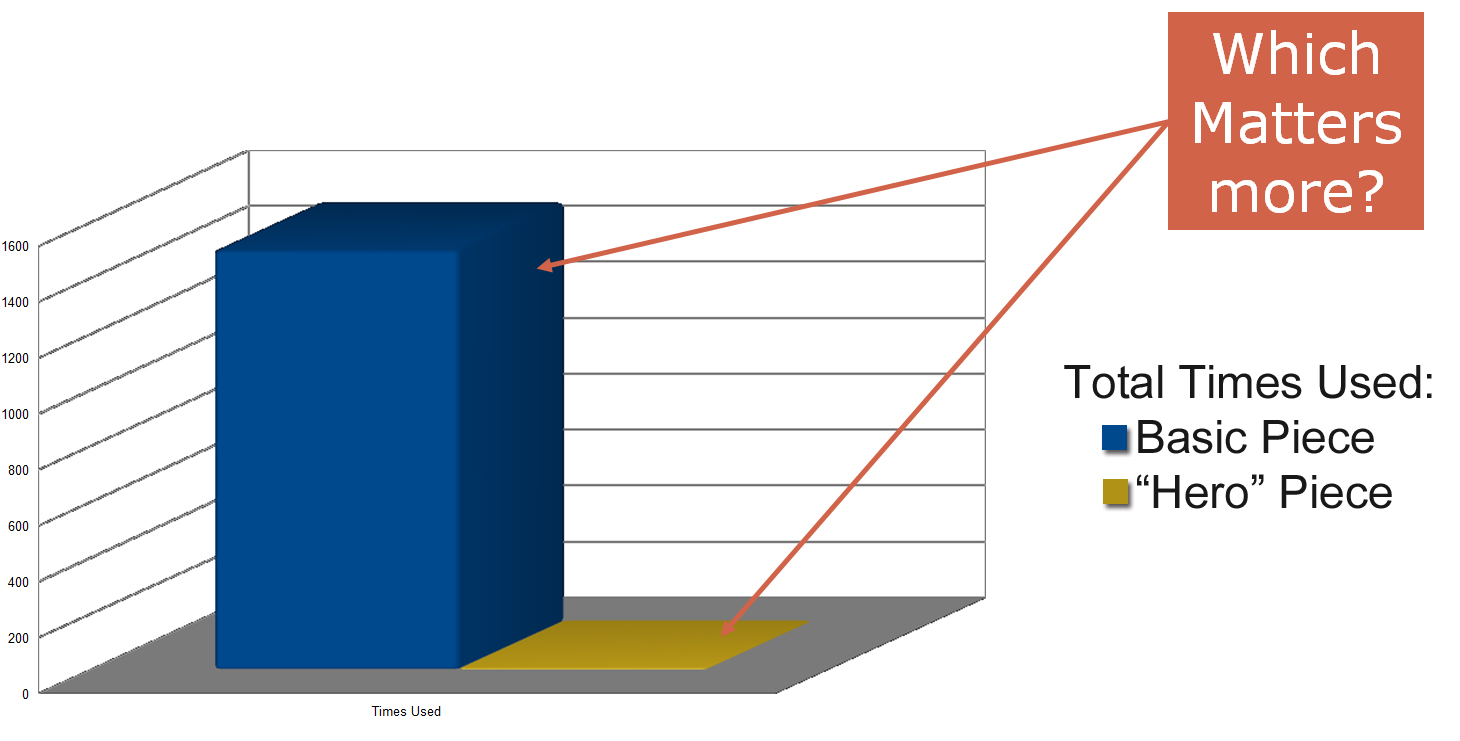
\includegraphics[scale = 0.23]{figures/HeroPieces}
		\caption{Por�wnanie czasu, jaki powinien zosta� po�wi�cony na tworzenie poszczeg�lnych asset�w (�r�d�o: \cite{Skyrim})}
	\end{figure}

\section{Tworzenie finalnej sceny i ustawianie o�wietlenia}
Podczas finalizowania procesu tworzenia poziomu projektanci skupiaj� si� g��wnie na jak najatrakcyjniejszym zaprezentowaniu stworzonej sceny. Kilkoma elementami nad kt�rymi warto skupi� si� w trakcie robienia tego s� mi�dzy innymi:
\begin{itemize}
	\item \textbf{Ukrycie niedoskona�o�ci przed oczami gracza}. Nie jest mo�liwe stworzenie mapy, kt�ra b�dzie idelna w ka�dym jej miejscu. Zawsze znajdzie si� jaki� punkt kt�ry jest wykonany troch� gorzej lub jest nieco mniej ciekawy ni� reszta poziomu. W takim wypadku dobrze jest schowa� je przed graczem. Aby to uzyska� stosuje si� takie techniki, jak:
	\begin{itemize}
		\item Zaciemnienie miejsca, kt�re chcemy ukry� - tam gdzie nie ma �wiat�a, nie mo�na dostrzec niedoskona�o�ci.
		\item Zas�oni�cie niedoskona�o�ci innymi obiektami - wszelkie �le spasowane elementy mo�na po prostu zas�oni� innym, pasuj�cym (mo�e to by� na przyk�ad g�az w jaskini albo s�up w �rodku budynku)
		\item Odwr�cenie uwagi gracza od takich miejsc - je�li gracz b�dzie mia� przed sob� inne, ciekawsze fragmenty poziomu istnieje mniejsza szansa na to, �e zwr�ci uwag� na te mniej doskona�e
	\end{itemize}
	Te wszystkie techniki mo�na ze sob� ��czy� w celu uzyskania jeszcze lepszego efektu.
	\item \textbf{Zwr�cenie uwagi gracza na elementy istotne w danym poziomie}. Tutaj chodzi przede wszystkim o to, aby gracz mia� ca�y czas �wiadomo�� tego dok�d musi i��, aby pchn�� dalej akcj�. Za pomoc� o�wietlenia mo�na go prowadzi� tak, aby pod��a� szlakiem wytyczonym przez tw�rc�w.
\end{itemize}
	\begin{figure}[!ht]
		\centering
		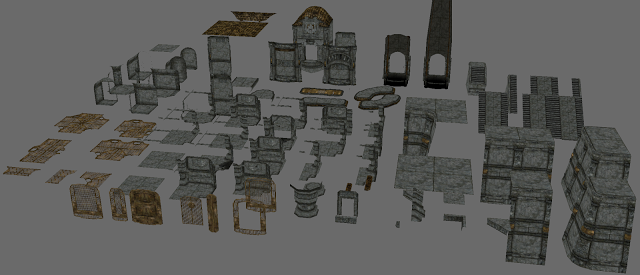
\includegraphics[scale = 0.73]{figures/Beta_models}
		\caption{Finalna paczka modeli (�r�d�o: \cite{Skyrim})}
	\end{figure}
































% !TeX encoding = windows-1250

\chapter{Realizacja cz�ci praktycznej}
\label{t:impementation}
Cz�� pracy dotycz�ca realizacji cz�ci praktycznej ma na celu pokazanie w jaki spos�b mo�na stworzy� paczk� modularnych asset�w stosuj�c si� do zasad opisanych we wcze�niejszych rozdzia�ach. Ka�dy z wykonanych krok�w zosta� pokazany za pomoc� opisu wykonania oraz poparty rysunkami i zrzutami ekranu pozwalaj�cymi zobaczy� efekt pracy. Nale�y jednak doda�, �e nie ka�dy z wymienionych wcze�niej krok�w zosta� wykonany w pe�ni zgodnie z jego opisem. Tyczy si� to zw�aszcza tych, kt�re dotyczy�y stricte pracy w wi�kszym zespole i mog�y zosta�y uproszczone lub zast�pione rozwi�zaniami bardziej pasuj�cymi do tworzenia bez wsp�pracownik�w.
\section{Inspiracja i �r�d�o grafiki koncepcyjnej}
Grafika koncepcyjna, jak i sam pomys� na stworzenie pracy zosta� zainspirowany comiesi�cznym wyzwaniem stawianym przed u�ytkownikami forum \textit{polycount.com}. Polega ono na jak najciekawszym odwzorowaniu fragmentu poziomu ukazanego na za��czonej grafice koncepcyjnej. Zasady konkursu s� do�� proste i zwykle aktywnie uczestniczy w nim przynajmniej kilka os�b z szerokiego grona u�ytkownik�w forum. Najwa�niejsze regu�y, kt�rych musz� trzyma� si� tw�rcy, to: \cite{NoobChallengeMay2015}
\begin{itemize}
	\item Prace musz� by� w ca�o�ci wykonane samodzielnie. Nie ma ogranicze� co do czasu stworzenia danego elementu, jednak nie wolno ich zapo�ycza� od innych tw�rc�w (ale mo�na wykorzystywa� tekstury wykonane nawet kilka miesi�cy wcze�niej w ramach innego projektu)
	\item Poziom musi zosta� zaprezentowany w dowolnym silniku gry komputerowej. Tw�rcy sugeruj� u�ycie \textit{CryEngine 3}, jednak bez �adnych przeszk�d mo�na wykorzysta� konkurencyjne technologie.
	\item Prac� nale�y uko�czy� przed up�yni�ciem narzuconego terminu (zwykle jest to 30 dni od daty publikacji postu na forum)
\end{itemize}
Dodatkowo, tw�rcy nie zalecaj� wykorzystywania program�w s�u��cych do szybkiego generowania asset�w. Przyk�adem takiego mo�e by� Quixel dDo - program pozwalaj�cy na generowanie tekstur r�nych powierzchni na podstawie wcze�niej stworzonych map (jak na przyk�ad normal mapa, kt�r� mo�na stworzy� za pomocn� innych program�w) oraz danych wprowadzonych przez u�ytkownika. \newline

Grafika koncepcyjna b�d�ca podstaw� realizacji cz�ci praktycznej pracy zosta�a zaczerpni�ta z jednej z edycji \textit{Monthly Community Noob Challenge}. W maju 2015 roku postawiono przed u�ytkownikami forum wyzwanie stworzenia wn�trza �wi�tyni. Obraz, na kt�rym wzorowali si� uczestnicy by� r�wnie� punktem wyj�cia dla realizacji tej pracy:
	\begin{figure}[!ht]
		\centering
		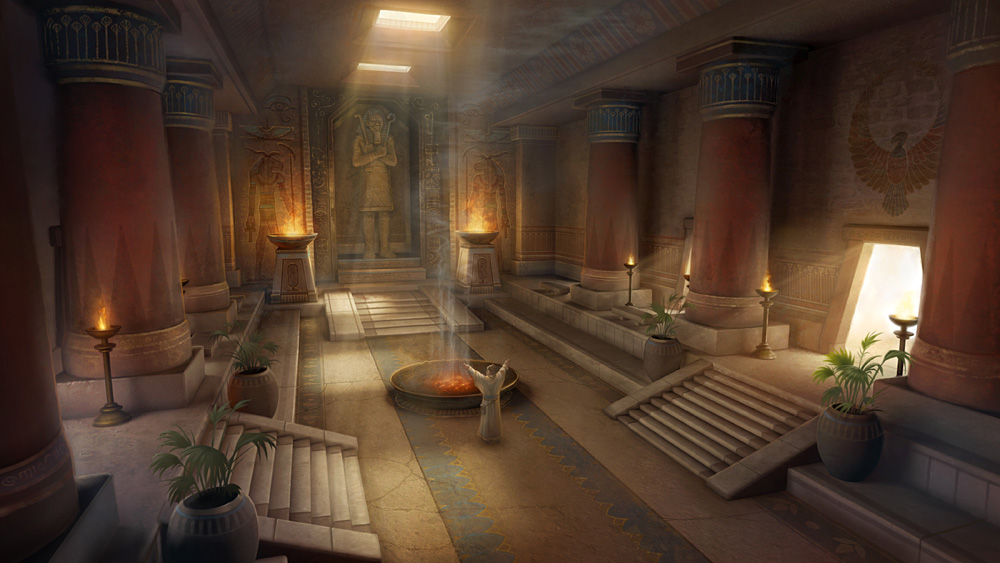
\includegraphics[scale = 0.45]{figures/My_concept}
		\caption{\textit{Monthly Community Noob Challenge 30} - grafika koncepcyjna (�r�d�o: \cite{NoobChallengeMay2015})}
	\end{figure}
\section{Faza projektowania}
Podczas preprodukcji szczeg�lny nacisk zosta� po�o�ony na opracowaniu takiego schematu dzia�ania, aby m�g� on zosta� w praktyce wdro�ony do pracy wi�kszego zespo�u i oszcz�dza� mo�liwie jak najwi�cej czasu podczas fazy produkcji. Przy tworzeniu pracy zosta�y wykorzystane narz�dzia nieprzystosowane do pracy w zespole, jednak te same metody mog� zosta� wykorzystane przy u�yciu innych program�w, kt�re zostan� zaproponowane podczas opisu realizacji. \newline

Pierwszym krokiem podczas fazy projektowej by� rozk�ad sceny na modu�y. Powsta�y w ten spos�b dwa nowe obrazki:
\begin{itemize}
	\item Podzia� z uwzgl�dnieniem modularnych modeli (przy czym pomini�to �ciany, sufity i pod�ogi dla zachowania lepszej czytelno�ci)
	\item Podzia� z uwzgl�dnieniem tekstur, kt�re znajd� si� w finalnym atlasie
\end{itemize}
Efekt pracy mo�na zobaczy� na rysunku 4.2.
	\begin{figure}[!ht]
		\centering
		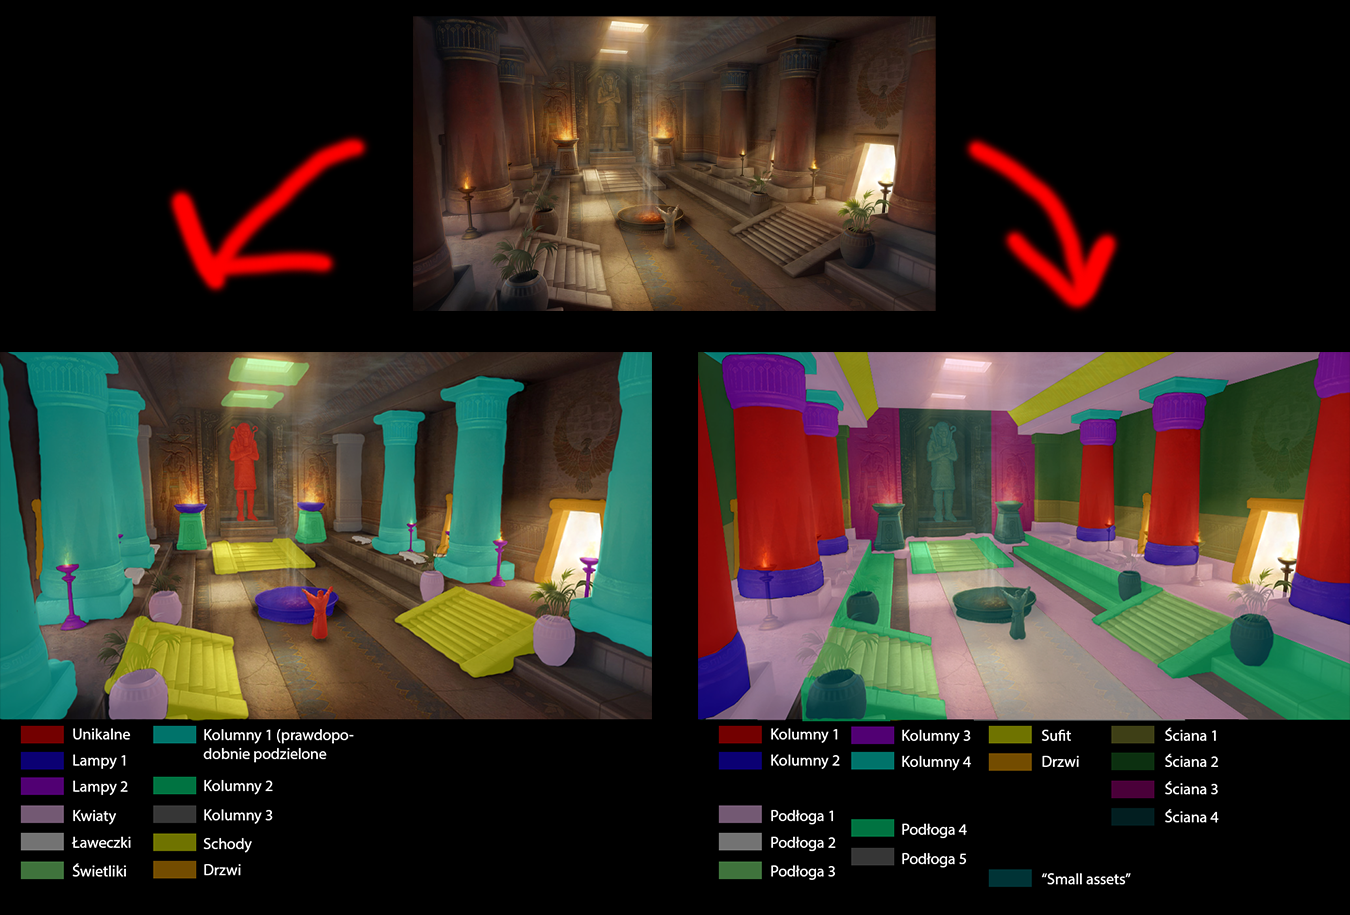
\includegraphics[scale = 0.30]{figures/My_breakdown}
		\caption{Podzia� na modularne modele i tekstury wybranej do realizacji grafiki koncepcyjnej (�r�d�o: opracowanie w�asne)}
	\end{figure}
	
Kolejnym etapem by�o utworzenie dokumentacji projektowej, kt�ra pozwala�aby na konsolidacj� procesu tw�rczego stosowanego przez zespo�y grafik�w i projektant�w. Tutaj szczeg�lny nacisk zosta� po�o�ony na odnalezieniu optymalnych rozwi�za� dla takiego zespo�u. \newline

\textbf{Stworzenie listy asset�w do wymodelowania i oteksturowania.} \newline 

Podczas tworzenia tej pracy zosta� wykorzystany pakiet \textit{LibreOffice}, kt�ry pozwala� na proste i logiczne posegregowanie ca�o�ci w arkuszu kalkulacyjnym. Utworzone zestawienia modeli i tekstur mo�na zobaczy� na rysunkach 4.3 oraz 4.4.
	\begin{figure}[!ht]
		\centering
		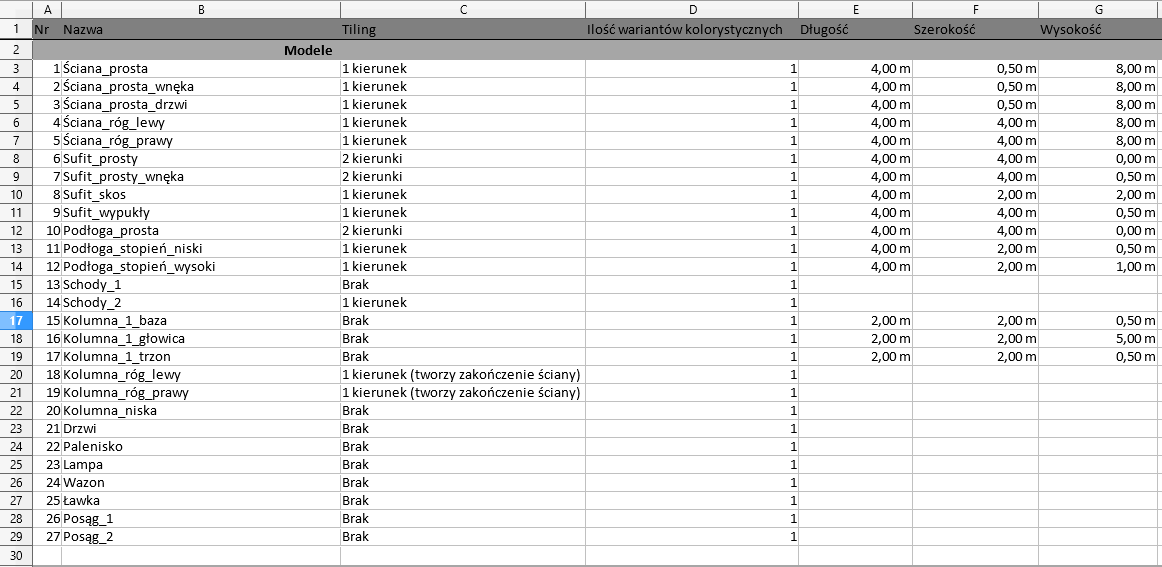
\includegraphics[scale = 0.50]{figures/Models_list}
		\caption{Lista modeli do wykonania podczas realizacji cz�ci praktycznej pracy (�r�d�o: opracowanie w�asne)}
	\end{figure}
	\begin{figure}[!ht]
		\centering
		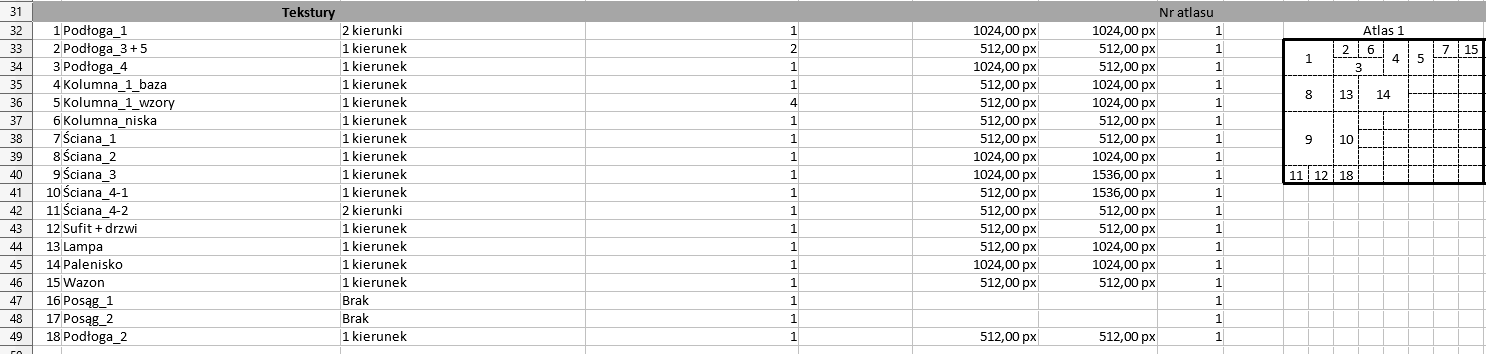
\includegraphics[scale = 0.40]{figures/Textures_list}
		\caption{Lista tekstur do wykonania podczas realizacji cz�ci praktycznej pracy (�r�d�o: opracowanie w�asne)}
	\end{figure}
	\newline
	Listy pokazane na obrazkach wymieniaj� kilka podstawowych parametr�w, kt�rych powinni trzyma� si� arty�ci podczas ich tworzenia. S� to w przypadku siatek 3d:
	\begin{itemize}
		\item Nazwa wst�pna (tutaj jeszcze niekoniecznie zgodna z nazewnictwem przyj�tym ostatecznie w silniku).
		\item Kierunek tilingu: tutaj wi�kszo�� siatek wykorzystuje jeden lub nie umo�liwia tilingu w og�le (jak na przyk�ad elementy ozdobne ustawiane swobodnie w scenie)
		\item Ilo�� wariant�w kolorystycznych: w przypadku modu��w wykorzystywanych wielokrotnie, liczba oznacza liczb� modeli wykonanych tak samo pod wzgl�dem geometrii, jednak r�ni�cych si� wygl�dem (przy zmianie parametr�w teksturowania, blendingu lub innych rozwi�zaniach pozwalaj�cych na urozmaicenie wygl�du siatek)
		\item Wymiary w scenie. Finalne rozmiary ka�dego z modeli (uwzgl�dniaj�ce skal� silnika i dopasowanie do gridu). Ma to na celu narzucenie grafikowi wymaga�, kt�re b�d� musia�y by� spe�nione przez ca�y czas tworzenia projektu. Dzi�ki temu mo�liwe b�dzie uk�adanie w scenie asset�w na bardzo wczesnym etapie produkcji.
	\end{itemize}
	Podczas tworzenia listy tekstur dodano jeszcze dwa aspekty, kt�re wcze�niej nie by�y istotne, a maj� wielkie znaczenie podczas tworzenia dwuwymiarowych grafik:
	\begin{itemize}
		\item Atlas tekstur, w kt�rym znalaz�a si� dana grafika. W przypadku tej pracy wszystkie grafiki zosta�y zamieszczone w jednym atlasie, jednak podczas tworzenia wi�kszych paczek cz�sto konieczny jest podzia� na kilka.
		\item Rozmieszczenie w danym atlasie. Takie podej�cie pokazuje dwie bardzo wa�ne rzeczy: jak obszerny jest atlas i ile wolnego miejsca pozosta�o na inne tekstury, a tak�e pozwala na wst�pne roz�o�enie koordynat�w UV obiekt�w zanim powstan� finalne tekstury wykorzystywane w paczce.
	\end{itemize}
	W przypadku tworzenia asset�w przez wi�kszy zesp�, taka lista mo�e zosta� podzielona na mniejsze fragmenty i udost�pniona jako zbi�r zada� do wykonania, a nast�pnie rozdzielona pomi�dzy poszczeg�lnych tw�rc�w za pomoc� narz�dzi takich, jak \textit{Trello} (dla ma�ych zespo��w), czy te� \textit{Redmine} (w przypadku bardziej rozbudowanych grup). \newline
	
	\textbf{Grid, parametry eksportu i nazewnictwo}. \newline
	
	Wszystkie tr�jwymiarowe modele wykorzystane w pracy zosta�y wymodelowane w programie \textit{Autodesk 3ds Max 2016}, z kt�rego nast�pnie eksportowano je do silnika 3d - \textit{Unreal Engine 4}. Poniewa� docelowa technologia domy�lnie stosuje system jednostek oparty o centymetry (1 unit w silniku to odpowiednik 1 cm), wymagane by�o dostosowanie ustawie� narz�dzi do modelowania dla wygodniejszej pracy. Domy�lna jednostka miary zosta�a zmieniona na 1 cm, a kolejne linie gridu zosta�y rozmieszczone co 100 cm. \newline
	
	Import modeli do \textit{Unreal Engine 4} odbywa si� poprzez pliki w formacie fbx, kt�re domy�lnie s� obs�ugiwane przez wi�kszo�� dost�pnych na rynku program�w do obr�bki grafiki tr�jwymiarowej. Silnik ma kilka wymaga� w kwestii parametr�w siatek, kt�re mo�e zaimportowa�. Najwa�niejsze z nich, to:
	\begin{itemize}
		\item W pliku �r�d�owym powinny znale�� si� grupy wyg�adzania dla ka�dej siatki.
		\item Jednostk� miary powinien by� centymetr, aby unikn�� ich skalowania.
	\end{itemize}
	Po dokonaniu zmian w ustawieniach eksportera, 3ds max umo�liwia zapisanie ich w postaci presetu. Pozwala to na szybkie przywr�cenie ustawie� w razie ich utraty oraz dystrybucj� pomi�dzy innych cz�onk�w zespo�u, gdy� pliki z presetami mo�na przenosi� mi�dzy komputerami. \newline
	
	Odpowiednie nazewnictwo jest bardzo wa�ne dla dobrej wsp�pracy na linii projektant - grafik modeluj�cy assety. W pracy wykorzystano nieco uproszczony system pochodz�cy z firmy Bethesda Softworks, kt�ry opisany by� w rozdziale trzecim. Wspomniane uproszczenie polega na nieu�ywaniu fragment�w odpowiedzialnych za wyr�nianie kilku warstw pakiet�w w kt�rym znajduje si� dany model oraz wyrzuceniu cz�ci dotycz�cej odbi� lustrzanych. Dodano r�wnie� rozdzielaj�cy poszczeg�lne cz�ony nazwy znak ''\_'', co ma na celu popraw� czytelno�ci. Przyk�adow� nazw� u�yt� dla siatki odwzorowuj�cej �cian� mo�na zobaczy� na rysunku 4.5:
		\begin{figure}[!ht]
			\centering
			
\includegraphics[scale = 1.30]{figures/My_naming}
			\caption{Przyk�adowa nazwa modelu w projekcie (�r�d�o: opracowanie w�asne)}
		\end{figure}
	Analiza poszczeg�lnych cz�on�w nazwy:
	\begin{itemize}
		\item \textbf{Shr} - stworzony pakiet zosta� nazwany ''Shrine'', co z angielskiego oznacza ''�wi�tynia'' - pierwsze trzy litery wyrazy pos�u�y�y do zgrupowania wszystkich modeli w jeden pakiet.
		\item \textbf{wall} - okre�la, �e jest to fragment �ciany
		\item \textbf{corn} - m�wi, �e element jest naro�nikiem
		\item \textbf{R} - okre�la kierunek, w kt�rym skr�ca naro�nik - w tym wypadku w prawo
		\item \textbf{mid} - kierunek tilingu - wertykalnie
		\item \textbf{02} - oznacza, �e jest to drugi wariant wizualny tego modelu
	\end{itemize}
\section{Faza prototypowania}
Szybkie, iteracyjne prototypowanie jest szczeg�lnie wa�ne, je�li chce si� unikn�� du�ych problem�w z ustawieniem obiekt�w w p�niejszych etapach projektu. Tutaj skupiono si� przede wszystkim na odpowiednim ustawieniem pivot�w dla ka�dego z nich. Modele i tekstury w tej fazie produkcji jeszcze dalekie s� od swojej finalnej formy, jednak po jej zako�czeniu nale�y pami�ta�, �e pewne parametry nie powinny zosta� ju� zmieniane do samego ko�ca projektu:
\begin{itemize}
	\item wymiary (d�ugo��, szeroko��, wysoko�� w przypadku siatek, po�o�enie w atlasie dla tekstur)
	\item pivoty
	\item nazwy
\end{itemize}
Kieruj�c si� t� zasad� zosta�y wytworzone modele gotowe do wst�pnego uk�adania w silniku. Dzi�ki temu �atwo jest unikn�� problem�w, gdy w wi�kszym zespole, w kt�rym r�wnolegle pracuj� zespo�y projektant�w i grafik�w praca jednych zostanie bardzo skomplikowana przez drugich. W takim wypadku warto r�wnie� umie�ci� informacje o umiejscowieniu pivot�w w dokumentacji projektowej (na przyk�ad na li�cie asset�w).  \newline

Na rysunku 4.6 mo�na zobaczy� przyk�adowe umiejscowienia pivot�w dla dw�ch modeli utworzonych podczas tej fazy. Pierwszy z nich (misa) ma go w �rodkowo-dolnej cz�ci, aby �atwo by�o go ustawia� w dowolnym miejscu na pod�odze. Jak �atwo zauwa�y� - jest to obiekt, w kt�rym wyb�r punktu opiera� si� o jego potencjalne u�o�enie w �rodowisku. W drugim z obiekt�w obrano miejsce przy dolnej kraw�dzi na pocz�tku siatki. Tutaj czynnikiem decyduj�cym by� tiling, gdy� jest to fragment �ciany, kt�ry musi idealnie pasowa� do innych podczas uk�adania w silniku.
	\begin{figure}[!ht]
		\centering
		\includegraphics[scale = 0.35]{figures/My_Pivots}
		\caption{Umiejscowienie pivot�w w zale�no�ci od zastosowania modelu (�r�d�o: opracowanie w�asne)}
	\end{figure}

\section{Faza finalizowania}
Ostatnia faza polega�a na dopracowywaniu pokazowej sceny w taki spos�b, aby sta�a si� ona jak najatrakcyjniejsza dla potencjalnego ogl�daj�cego. Najwa�niejszymi zabiegami, kt�re zosta�y tutaj zastosowane by�y:
\begin{itemize}
	\item \textbf{Dopasowanie parametr�w materia��w wykorzystanych w projekcie} \newline
	Odpowiednie sparametryzowanie materia��w pozwala na uzyskanie lepszych efekt�w wizualnych, w zale�no�ci od zamiar�w tw�rcy. \textit{Unreal Engine 4} pozwala chocia�by na zmianie szorstko�ci materia�u, intensywno�ci emisji, czy te� prze�roczysto�ci. Ich odpowiednie ustawienie pozwala na osi�gni�cie wi�kszego realizmu. Odnalezienie odpowiedniego kompromisu pomi�dzy poziomem komplikacji materia��w, a efektem wizualnym jest wi�c kluczowe dla jako�ci pakietu. \newline
	
	W zaprezentowanej pracy skupiono si� g��wnie na odpowiednim zaznaczeniu rodzaju materia�u, kt�rego u�ywa dana powierzchnia (a w szczeg�lno�ci na parametrze metalness, kt�ry odpowiada za jego ''metaliczno��'').\newline
	\item \textbf{Dodanie efekt�w graficznych} \newline
	Efekty graficzne pozwalaj� na dodatkowe wzbogacenie sceny. Dobrym przyk�adem jest tu wykorzystanie efekt�w cz�steczkowych (ang. particle effects) do ''o�ywienia'' sceny. Przyk�adowo - poziom wykonany podczas realizacji projektu zawiera w sobie p�on�ce znicze; efekt ten zosta� uzyskany dzi�ki wykorzystaniu wy�ej wymienionej techniki.\newline
	
	Innym efektem, kt�ry warto tu wspomnie� jest postprocessing sceny. Efekty, takie jak rozmycie (ang. blur), czy okluzja otoczenia (ang. ambient oclussion) pozwalaj� na poprawienie finalnego efektu. Nale�y jednak pami�ta�, �e ich wykorzystywanie czasami znacznie zwi�ksza zapotrzebowanie na zasoby komputera podczas renderowania sceny.\newline
	\item \textbf{Dodanie o�wietlenia} \newline
	We wcze�niejszych rozdzia�ach wspomniane by�o kilkukrotnie o tym, jak wa�ne jest odpowiednie o�wietlenie poziomu. Pozwala ono na oddanie odpowiedniego klimatu dla sceny oraz na wyeksponowanie lub ukrycie pewnych jego fragment�w. \newline
	
	W pracy wykorzystano ��tawo-pomara�czowe o�wietlenie, kt�re dobrze oddaje klimat pomieszcze� o�wietlanych przy pomocy otwartego ognia. Dodatkowo - zastosowanie niewielkiej intensywno�ci jeszcze bardziej wzmacnia ten efekt. Por�wnanie poziomu z ustawionym w scenie i wypieczonym przez silnik o�wietleniem mo�na zobaczy� na rysunku 4.7.
	\begin{figure}[!ht]
		\centering
		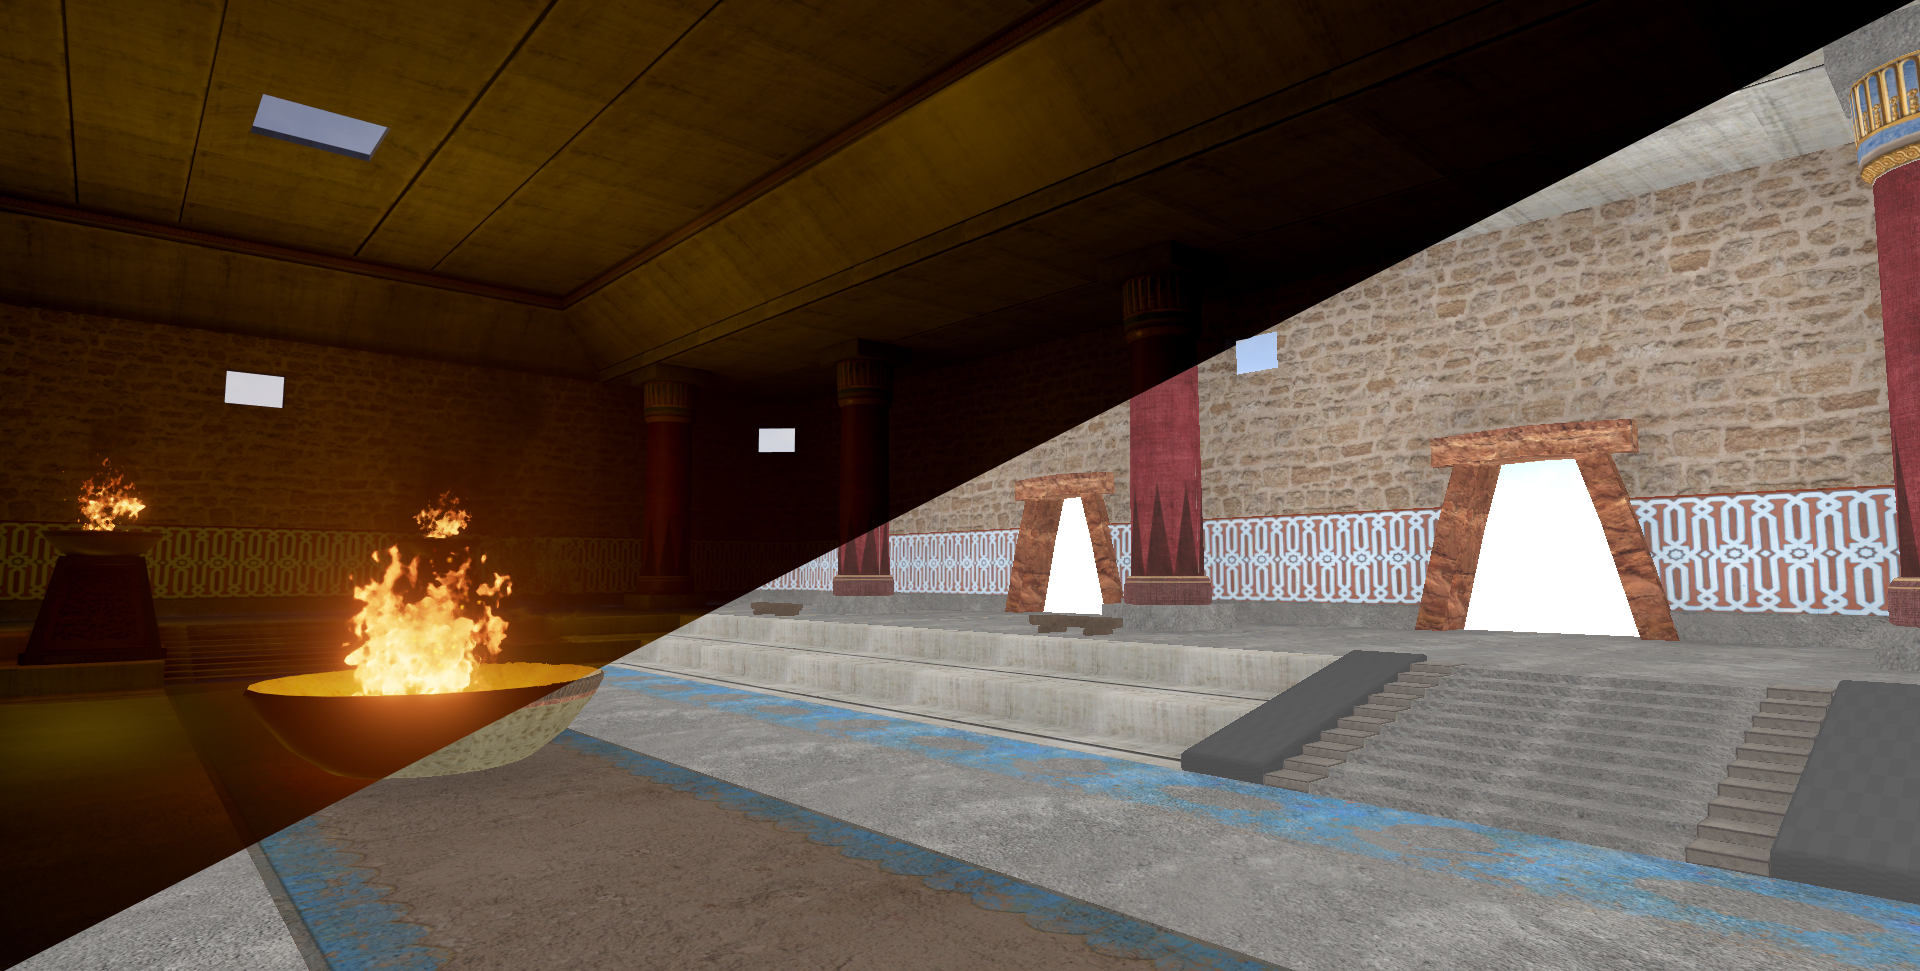
\includegraphics[scale = 0.30]{figures/lighting_comparsion}
		\caption{Por�wnanie sceny przed i po ustawieniu o�wietlenia (�r�d�o: opracowanie w�asne)}
	\end{figure}
\end{itemize}
Kieruj�c si� wytycznymi wyznaczonymi na wcze�niejszych etapach pracy powsta� pakiet 40 tr�jwymiarowych modeli oteksturowanych przy pomocy 3 atlas�w w rozdzielczo�ci 4096 na 4096 pikseli (po jednym atlasie dla map diffuse, normal i roughness). Zrzut ekranu z programu \textit{3ds Max 2016} prezentuj�cy wszystkie wymodelowane siatki wielok�towe (wraz z teksturami na nich) mo�na zobaczy� na rysunku 4.8.
\begin{figure}[!ht]
	\centering
	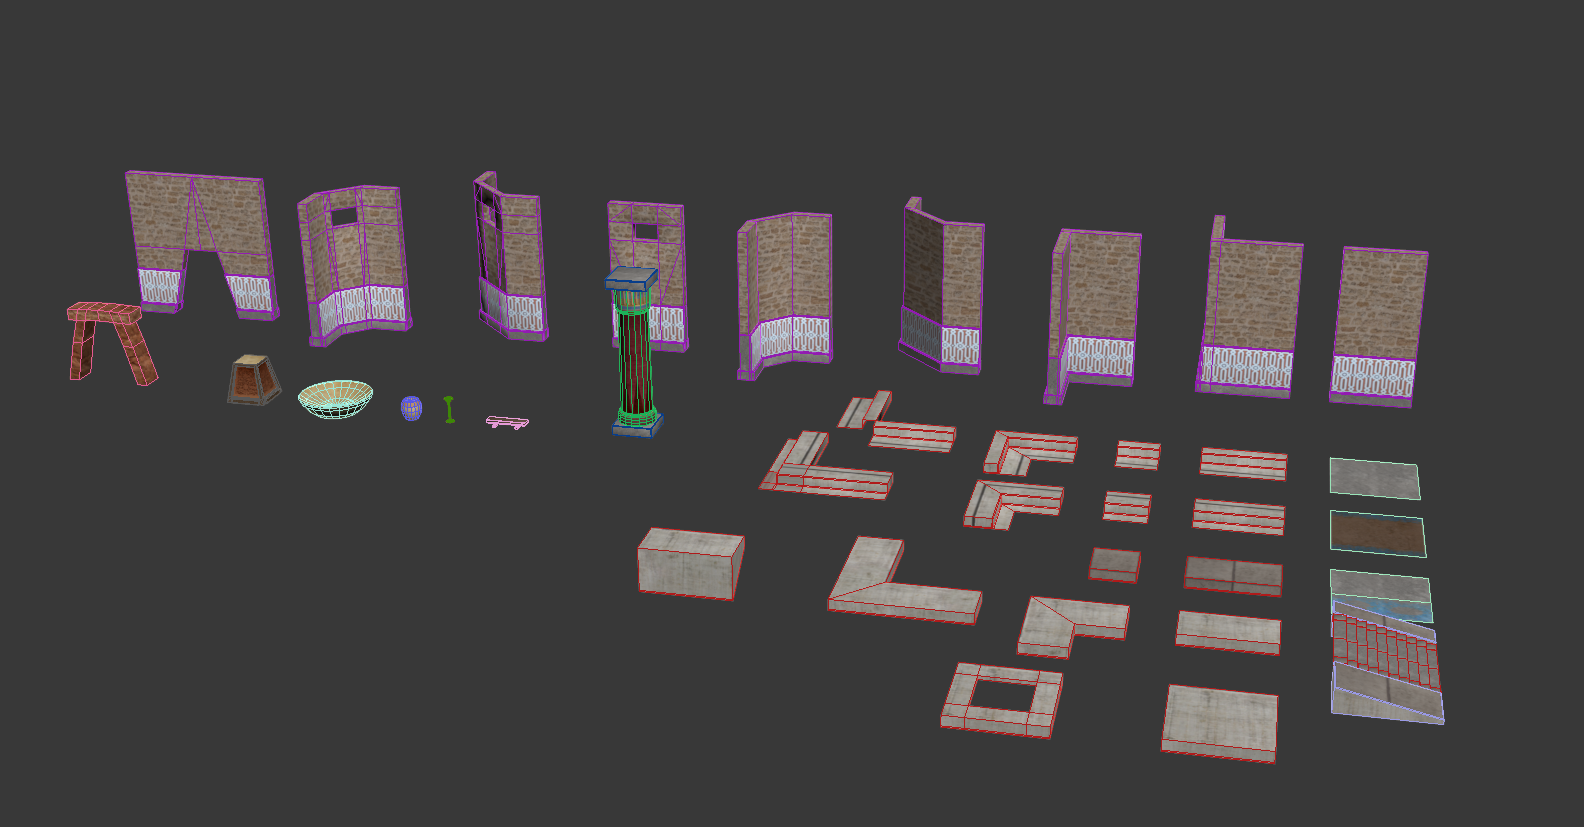
\includegraphics[scale = 0.35]{figures/My_assets_pack}
	\caption{Modele stworzone na potrzeby projektu (�r�d�o: opracowanie w�asne)}
\end{figure}

Z ukazanych wy�ej asset�w powsta�a scena wzorowana na wybranej wcze�niej grafice koncepcyjnej. Por�wnanie efektu uzyskanego w trakcie realizacji pracy z punktem wyj�ciowym zosta�o ukazane na rysunku 4.9.
\begin{figure}[!ht]
	\centering
	\includegraphics[scale = 0.25]{figures/Comparsion_with_concept}
	\caption{Por�wnanie grafiki koncepcyjnej ze scen� utworzon� podczas realizacji cz�ci praktycznej pracy (�r�d�o: opracowanie w�asne)}
\end{figure}

Przestrze� utworzon� w tej pracy dodatkowo ukazuj� ilustracje 4.10 oraz 4.11. Natomiast na rysunku 4.12 zawarto przyk�ad detalu - lampionu z efektem cz�steczkowym p�omienia.
\begin{figure}[!ht]
	\centering
	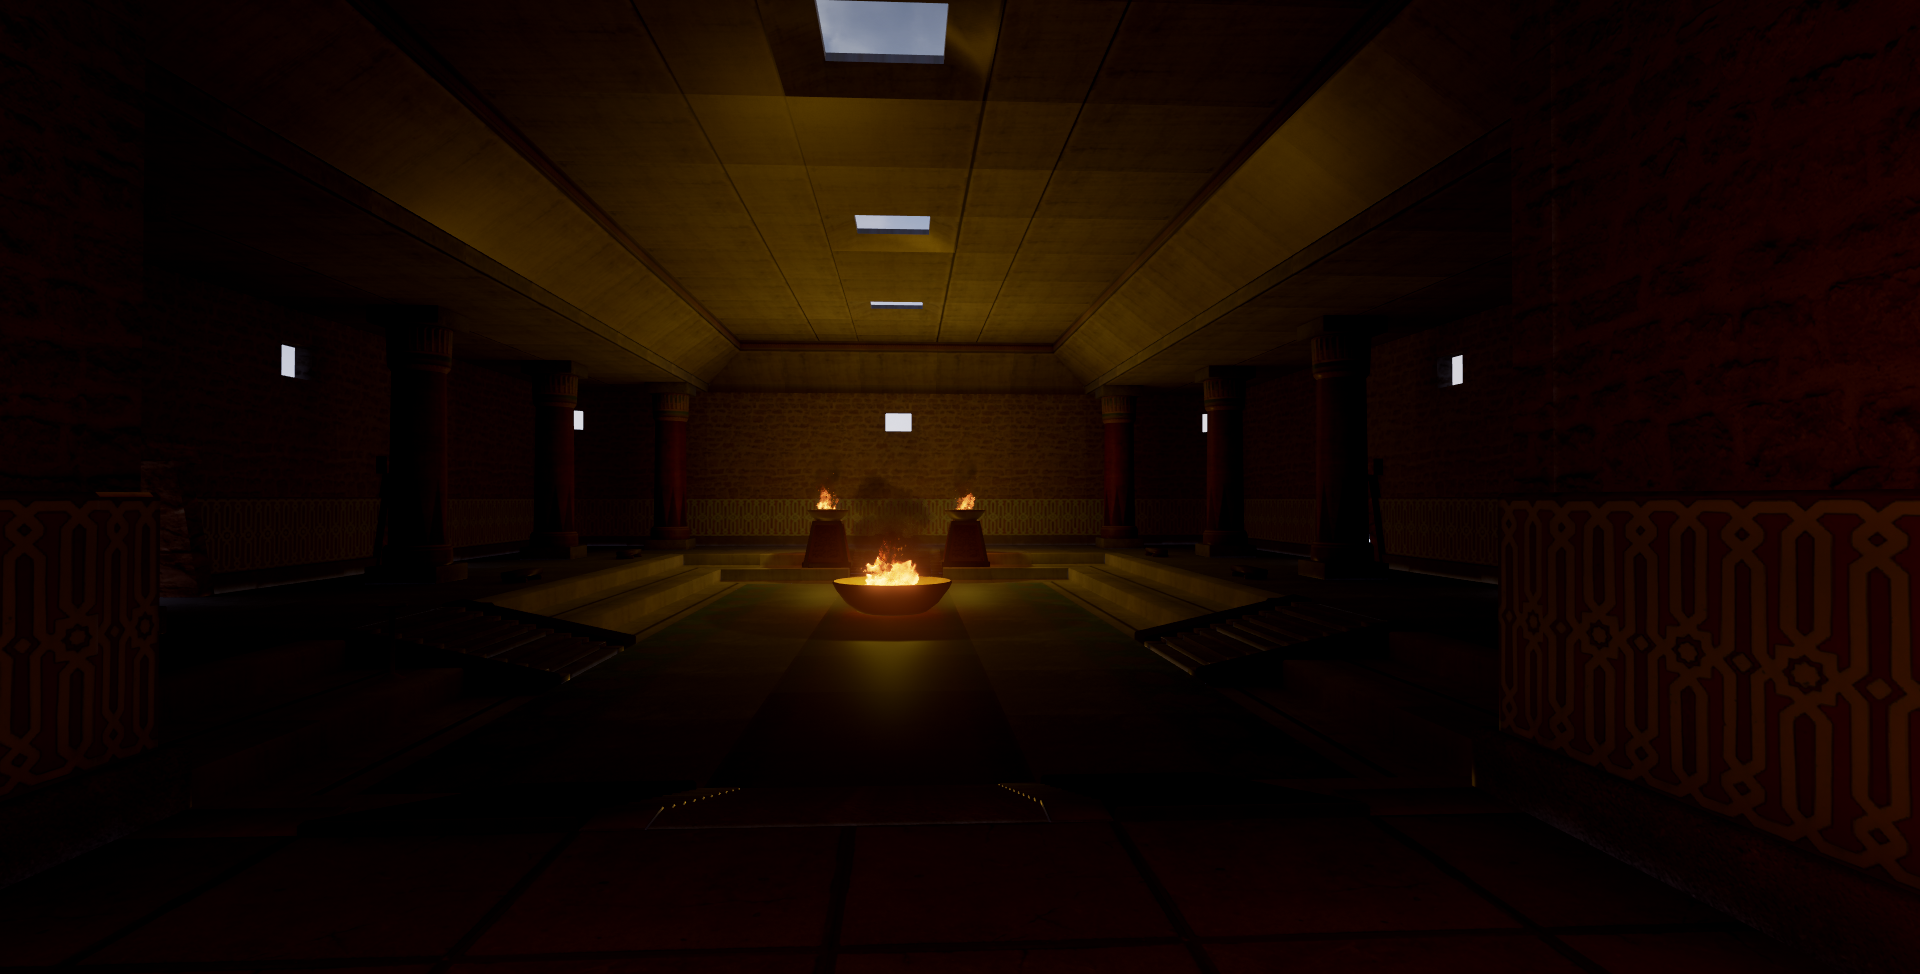
\includegraphics[scale = 0.20]{figures/space}
	\caption{Scena z perspektywy wej�cia niewidocznego na grafice koncepcyjnej (�r�d�o: opracowanie w�asne)}
\end{figure}
\begin{figure}[!ht]
	\centering
	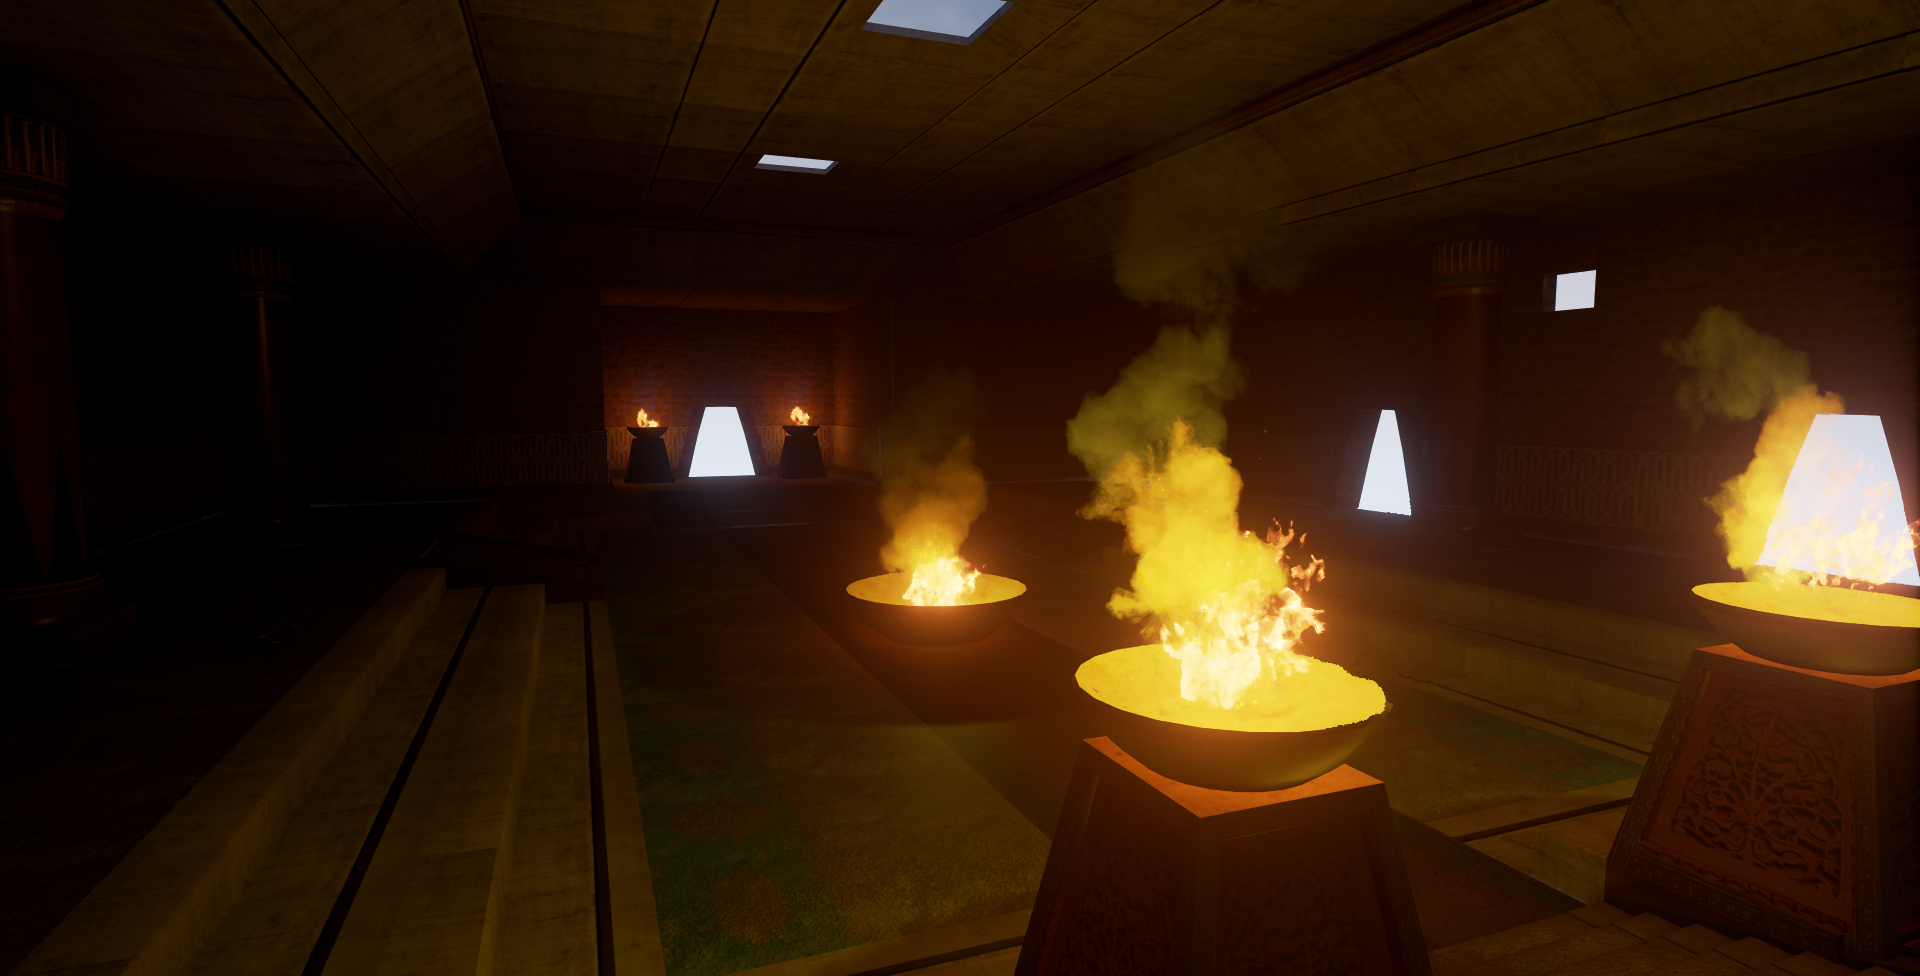
\includegraphics[scale = 0.20]{figures/persp_1}
	\caption{Scena z perspektywy ukazuj�cej niewidoczn� na grafice koncepcyjnej cz�� �wi�tyni (�r�d�o: opracowanie w�asne)}
\end{figure}
\begin{figure}[!ht]
	\centering
	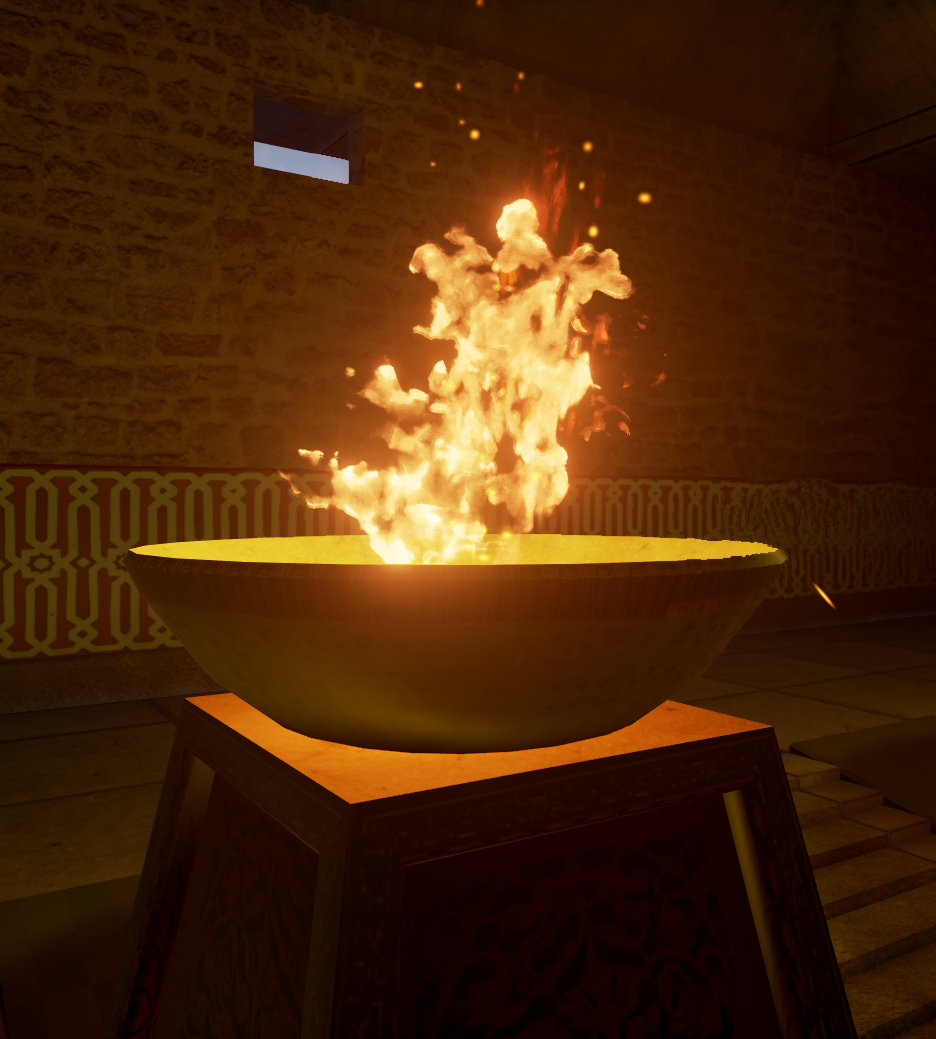
\includegraphics[scale = 0.20]{figures/detail}
	\caption{P�on�cy lampion widoczny z bliskiej odleg�o�ci (�r�d�o: opracowanie w�asne)}
\end{figure}
% !TeX encoding = windows-1250

\chapter{Podsumowanie i wnioski}
\label{t:conslusions}


% !TeX encoding = windows-1250
\begin{thebibliography}{999}
	\bibitem{MostInfluentialGames} 15 Most Influential Games of All Time, \emph{Virtua Racing � Arcade (1992)}, \newline\texttt{https://web.archive.org/web/20100412225953/http://www.gamespot.com/gamespot\newline/features/video/15influential/p13\_01.html}, witryna internetowa, stan na 28 lipca 2016
	
	\bibitem{Investigation} S. Jones, \emph{Investigation into modular design within computer games}, praca licencjacka, Uniwersytet Staffordshire, 2011
	
	\bibitem{CreatingModularGameArt} Creating Modular Game Art For Fast Level Design, \texttt{http://www.gamasutra.com/view/feature/130885\newline/creating\_modular\_game\_art\_for\_fast\_.php}, witryna internetowa, stan na 31 lipca 2016
\end{thebibliography}


\listoffigures

% !TeX encoding = windows-1250

\chapter*{Abstract}



\newpage
\thispagestyle{empty}
\begin{textblock}{1}(-2.65,-1.65)
	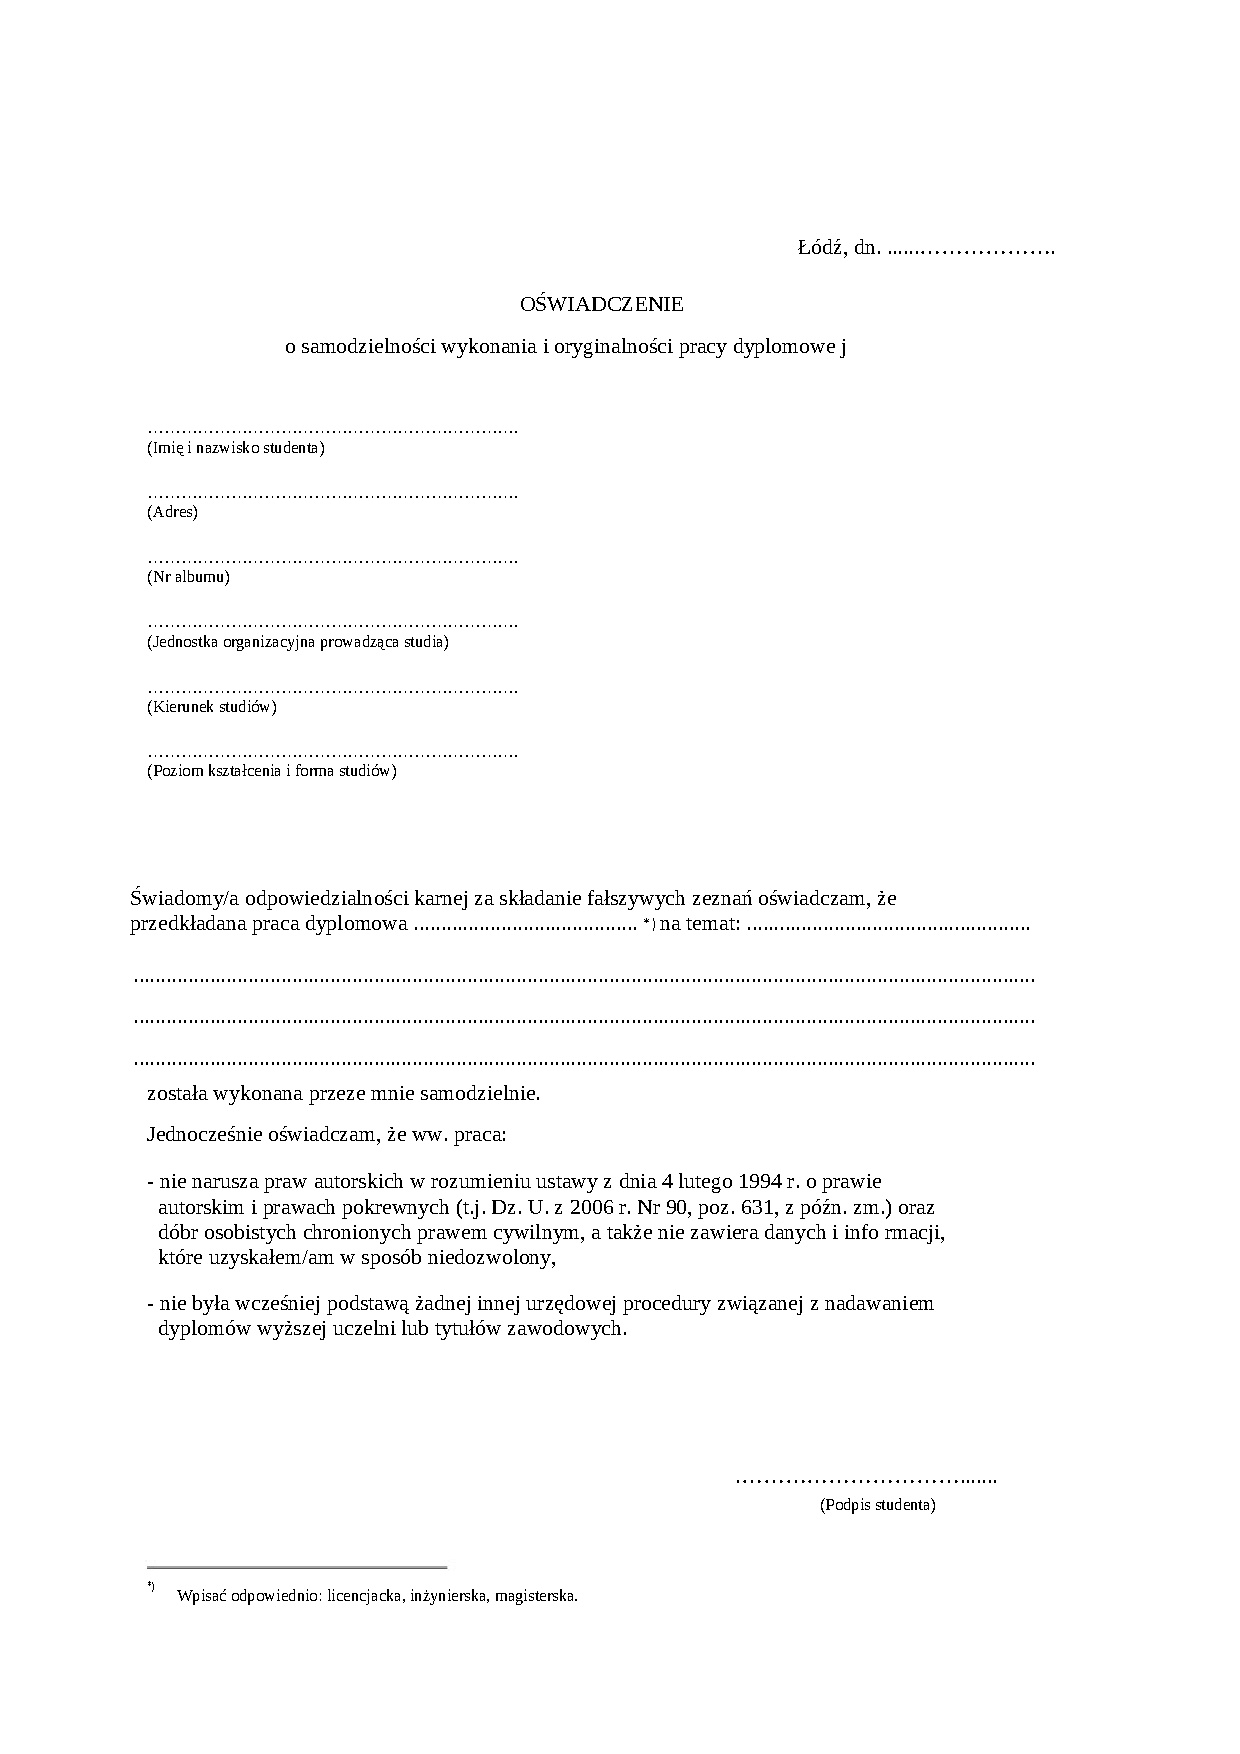
\includegraphics{figures/Zal_2.pdf}
\end{textblock}

\end{document}
